\documentclass[sigconf]{acmart}
\let\Bbbk\relax
\usepackage{amssymb}
\usepackage{amsfonts}
\usepackage{graphicx}
\usepackage{bbm}
\usepackage{diagbox}
\usepackage{algpseudocode}
\usepackage{amsmath}
\usepackage{float}
\usepackage{tabularx}
\usepackage{slashed}
\usepackage{algorithm}
\usepackage{algorithmicx} 
\usepackage{subfigure}
\usepackage{libertine}
\usepackage{tikz}
\usepackage{verbatim}
\usepackage{tablefootnote}
\usepackage{enumitem}
\usepackage{color}

\AtBeginDocument{
  \providecommand\BibTeX{
        {
            \normalfont B
            \kern-0.5em
            {
                \scshape i
                \kern-0.25em b
            }
            \kern-0.8em
            \TeX
        }
    }
}
\newtheorem{Definition}{Definition}
\newtheorem*{Theorem}{Theorem}
\newtheorem*{Proof}{Proof}
\newtheorem{Lemma}{Lemma}
\newtheorem{Example}{Example}

\def\ojoin{\setbox0=\hbox{$\bowtie$}%
  \rule[0.15ex]{.25em}{.4pt}\llap{\rule[0.95ex]{.25em}{.4pt}}}
\def\leftouterjoin{\mathbin{\ojoin\mkern-5.8mu\bowtie}}
\def\rightouterjoin{\mathbin{\bowtie\mkern-5.8mu\ojoin}}
\def\fullouterjoin{\mathbin{\ojoin\mkern-5.8mu\bowtie\mkern-5.8mu\ojoin}}

%\setcopyright{acmcopyright}
%\copyrightyear{2022}
%\acmYear{2022}
%\acmDOI{10.1145/1122445.1122456}

%% These commands are for a PROCEEDINGS abstract or paper.
%\acmConference[Woodstock '18]{Woodstock '18: ACM Symposium on Neural Gaze Detection}{June 03--05, 2018}{Woodstock, NY}
%\acmBooktitle{Woodstock '18: ACM Symposium on Neural Gaze Detection, June 03--05, 2018, Woodstock, NY}
%\acmPrice{15.00}
%\acmISBN{978-1-4503-XXXX-X/18/06}

%%
%% Submission ID.
%% Use this when submitting an article to a sponsored event. You'll
%% receive a unique submission ID from the organizers
%% of the event, and this ID should be used as the parameter to this command.
%%\acmSubmissionID{123-A56-BU3}

%%
%% The majority of ACM publications use numbered citations and
%% references.  The command \citestyle{authoryear} switches to the
%% "author year" style.
%%
%% If you are preparing content for an event
%% sponsored by ACM SIGGRAPH, you must use the "author year" style of
%% citations and references.
%% Uncommenting
%% the next command will enable that style.
%%\citestyle{acmauthoryear}

%%
%% end of the preamble, start of the body of the document source.
%\citestyle{acmauthoryear}

\begin{document}

\title{Discarding Global Plan Makes Re-optimization Better}

\author{Junyi Zhao}
\email{zhaojy20@mails.tsinghua.edu.cn}
\affiliation{%
  \institution{Institute for Interdisciplinary Information Science, Tsinghua University}
  \city{Beijing}
  \country{China}
}

\author{Yihan Gao}
\email{gaoyihan@mail.tsinghua.edu.cn}
\affiliation{%
    \institution{Institute for Interdisciplinary Information Science, Tsinghua University}
    \city{Beijing}
    \country{China}
}

\begin{abstract}
    \input{1_Abstract.tex}
\end{abstract}

%%
%% The code below is generated by the tool at http://dl.acm.org/ccs.cfm.
%% Please copy and paste the code instead of the example below.
%%
%\begin{CCSXML}
%    <ccs2012>
%     <concept>
%      <concept_id>10010520.10010553.10010562</concept_id>
%     <concept_desc>Computer systems organization~Embedded systems</concept_desc>
%      <concept_significance>500</concept_significance>
%     </concept>
%     <concept>
%      <concept_id>10010520.10010575.10010755</concept_id>
%      <concept_desc>Computer systems organization~Redundancy</concept_desc>
%      <concept_significance>300</concept_significance>
%     </concept>
%     <concept>
%      <concept_id>10010520.10010553.10010554</concept_id>
%      <concept_desc>Computer systems organization~Robotics</concept_desc>
%     <concept_significance>100</concept_significance>
%     </concept>
%     <concept>
%      <concept_id>10003033.10003083.10003095</concept_id>
%      <concept_desc>Networks~Network reliability</concept_desc>
%      <concept_significance>100</concept_significance>
%     </concept>
%    </ccs2012>
%    \end{CCSXML}
    
%    \ccsdesc[500]{Computer systems organization~Embedded systems}
%   \ccsdesc[300]{Computer systems organization~Redundancy}
%    \ccsdesc{Computer systems organization~Robotics}
%    \ccsdesc[100]{Networks~Network reliability}

\maketitle

\section{Introduction} \label{S1}
    \textcolor{blue}{
    Cardinality estimation (CE) is essential for cost-based query optimization because cardinality is used in the cost model. The error in cardinality estimation may lead the cost-based optimizer to sub-optimal plans.
}\par
\textcolor{blue}{
    Histogram-based cardinality estimation can make mistakes on complex queries due to the correlations in the predicates and the increasing estimation error with join size \cite{paper31}. However, such cardinality estimation method remains dominant in practice because of its low overhead. Many ideas have been raised to address the issue of cardinality estimation error, for example, samples \cite{paper19, paper22, paper23}, sketches \cite{paper55, PessimisticCE}, graphical models \cite{paper5}, and even machine learning \cite{MLCE}. However, they still cannot replace histogram-based ones because of their high online overhead or great efforts for pre-processing \cite{SampleReopt}.
}\par
    As it is challenging to solve the cardinality estimation problem \cite{MichaelStonebraker}, re-optimization \cite{Reopt, Pop, MichaelStonebraker, SampleReopt, QIE} is proposed to avoid the need for accurate cardinality estimation. Re-optimization first generates an initial execution plan at the beginning and then detects during run-time whether the actual behavior of a query plan becomes significantly different from what was expected. Then, re-optimization attempts to correct the execution plan whenever a significant deviation is found. In most implementations, re-optimization materializes a sub-tree of the global plan tree (sub-plan) and uses the statistics collected after materialization to refine the remaining part.\par
\textcolor{blue}{
    However, a problem with the current re-optimization techniques is that they rely heavily on the global plan. More specifically, re-optimization always chooses a sub-tree of the global plan to materialize. We call this way of re-optimization the sub-plan perspective. The problem is, due to the cardinality estimation error, the global plan is always far away from the optimal plan. Therefore, the terrible global plan influences the quality of the sub-plan. At its worst, the first few execution steps of the global plan may be bad decisions, and they cannot be corrected by re-optimization. For example, suppose the first-executed sub-plan deteriorates the execution time of the remaining query. It is impossible to correct that case because re-optimization will be triggered after this sub-optimal plan is executed.
}\par
\textcolor{blue}{
    To tackle the problem of current re-optimization, we propose a new re-optimization framework called \textit{query split}. Unlike traditional re-optimizations, \textit{query split} is designed in a sub-query perspective. Specifically, for select-projection-join (SPJ) queries, we first split them into several sub-queries before query optimization, then optimize and execute them sequentially to get the result of the original query. After materializing the sub-query results, we collect run-time statistics and use them in the query optimization for other sub-queries. From the sub-query perspective, we avoid the misleading global plan and decrease the problem scale of query optimization. As shown later in this paper, we get better execution plans than the sub-plan perspective by a proper sub-query splitting strategy.
}\par
\textcolor{blue}{
    Besides, the sub-query perspective provides a more robust overhead of materialization. In traditional query re-optimization, the times of materialization are unknown, depending on the current plan. For example, in mid-query re-optimization \cite{Reopt}, materialization happens at those blocked operators (e.g., sort and hash). In \textit{Pop} \cite{Pop}, materialization can also occur at the outer sides of the nest-loop join. This reactive pattern leads to too much or too little materialization overhead. In contrast, \textit{query split} decides where to materialize as soon as the query comes, decreasing the potential extreme overhead of materialization.
}\par
    Our experiment shows that \textit{query split} with the sub-query perspective beats sketch-based cardinality estimation approaches and traditional re-optimization on Join Order Benchmark \cite{JOB}. Moreover, \textit{query split} with the sub-query perspective can get an end-to-end latency which is very close to optimal.\par
\textcolor{blue}{
    The contribution of this paper can be summarized as follows:
    \begin{enumerate}[leftmargin = 15pt]
        \item We propose a new perspective for re-optimization called the sub-query perspective, which is opposite to the traditional sub-plan perspective. Sub-query perspective leads to a better plan for each sub-query and avoids the potential high overhead of materialization.
        \item We propose a re-optimization framework called \textit{query split} to cooperate with our sub-query perspective.
        \item Experimental results showed that \textit{query split} significantly outperformed existing approaches.
    \end{enumerate}
}\par
The rest of the paper is organized as follows. Section \ref{S2} motivates the sub-query perspective and \textit{query split}. Section \ref{S3} formally describes \textit{query split} and proves its correctness. Section \ref{S4} shows preliminary implementations of \textit{query split} with the sub-query perspective. Section \ref{S5} evaluates the performance of the \textit{query split}. Section \ref{S6} discusses how to extend \textit{query split} to general query forms. Section \ref{S7} gives a case study on \textit{query split} for a deep insight. Finally, Section \ref{S8} discusses related works, and Section \ref{S9} concludes this paper.
    
\section{Motivation} \label{S2}
    \textcolor{blue}{
    This section consists of three main parts. The first part is that we motivate the importance of re-optimization. Then, we characterize the fundamental limitation of traditional re-optimization. Last, we use it as motivation to introduce a new perspective of re-optimization called the sub-query perspective and a novel query processing framework called \textit{query split}.
}
    \begin{itemize}[leftmargin = 15pt]
        \item We first review the problem of cardinality estimation and explain why it is hard to accurately estimate the cardinality of complex query results (in Section \ref{S21}).
        \item Then, we review an existing query processing technique called re-optimization and discuss the underlying philosophy of re-optimization (in Section \ref{S22}).
    \textcolor{blue}{
        \item Next, we discuss shortages of the sub-plan perspective, which traditional re-optimization methods adopt (in Section \ref{S23}).
        \item Last, we propose a new perspective of re-optimization called the sub-query perspective and design a \textit{query split} framework to cooperate with this new perspective (in Section \ref{S24}).
    }
    \end{itemize}

\subsection{Intrinsic Difficulty of Cardinality Estimation} \label{S21}
    Currently, most database systems estimate cardinality as the product of three terms: the size of both relations and predicate selectivity, in which the selectivity is estimated via table statistics \cite{book1}. For example, in PostgreSQL, the selectivity of a simple predicate on base tables is estimated using gathered statistics such as histograms, most common values and their frequencies, and the number of distinct values. For conjunctive predicates, it is commonly assumed that the component predicates are independent, so the final selectivity is the product of the selectivity of each predicate \cite{JOB}. For complex join queries, independence between join predicates is often assumed, and their selectivities are multiplied together. In MySQL, the cardinality estimation strategy is very similar \cite{manual1}.\par
    There are two major reasons why it is hard to guarantee the accuracy of cardinality estimation \cite{Reopt}. The first reason is that optimizer lacks the statistics of intermediate relations. We use an example to demonstrate why this is a problem that troubles the optimizer.
    \begin{Example}
        A database contains two relations $A(a)$ and $B(a, b)$ and some statistics in the system catalog including the cardinality of two relations $n_A$ and $n_B$ and the value distribution of attributes $f_A^a$, $f_B^a$ and $f_B^b$. Given a natural join query $r=A \bowtie B$, the cardinality of $r$ is given by:\par
        $n_r=n_A \times n_B \times selec_{A,B}=n_A \times n_B \times \Sigma_{i \in dom(a)}(f_A^a(i) \times f_B^a(i))$
        where $dom(a)$ is the domain of attributes $a$.\par
        However, when we apply a filter to attribute $b$, cardinality estimation of $r$ becomes more difficult. Consider the query $r=A \bowtie \sigma_{b=x}(B)$, and denote the intermediate relation as $t=\sigma_{b=x}(B)$. So that the query can be rewritten as $r=A \bowtie t$, and the cardinality of $t$ is $n_t=n_B \times f_B^b(x)$. Since any other statistic about $t$ is unknown, the optimizer must approximate those missing statistics by some assumptions. For example, if we assume independence between attributes $a$ and $b$ in table $B$, we can get $f_t^a(i) = f_B^a(i|b=x) = f_B^a(i)$, which can then be used to estimate the selectivity of join predicate. However, those assumptions may not be actually valid, and would introduce error in estimation.\par
        Similar situation happens when the filter $\sigma_{b=x}(B)$ is replaced by a new join, e.g. $r=A \bowtie (B \bowtie C)$. Since we only have the statistics of base relations, to estimate the cardinality of the final result $n_r$, we have to assume independence across joins. Specifically, we use the selectivity of joins between base relations to approximate the selectivity of joins containing intermediate results, which also leads to estimation error.
    \end{Example}
    From the above example, we can see that the optimizer has to make assumptions to compensate for the lack of statistics, which inevitably generates estimation errors.\par
    The second reason is error propagation. Yannis and Stavros mathematically deduce that the cardinality estimation error of an N-way natural join grows exponentially with N, assuming that there is some error in estimating the distribution of join attribute in each relation \cite{paper31}. Hence, except for small queries, cardinality estimation results are often not trustworthy. Although these results are based on theoretical analysis, they are also generally valid in practice based on our empirical observations during experiments.\par

\subsection{Re-optimization} \label{S22}
    As it is hard to make cardinality estimation always accurate, Kabra and DeWitt proposed re-optimization \cite{Reopt} to circumvent this problem. Re-optimization collects statistics during run-time to monitor query execution. When the collected statistics deviate too much from prediction, the system replans the remainder of the query plan in light of this new information, which can alter join orders and physical operators of the remaining part.\par
    As shown in Figure \ref{F1}, in a re-optimization scheme, the optimizer initially provides an execution plan to be executed. Then, during the execution of the plan, we materialize the intermediate result and switch back to the optimizer with some new run-time statistics collected during materialization. With such information, the optimizer can either keep the original plan or produce another plan to be executed. This iteration can happen several times until the final result is ready.\par
    \begin{figure}
        \centering
        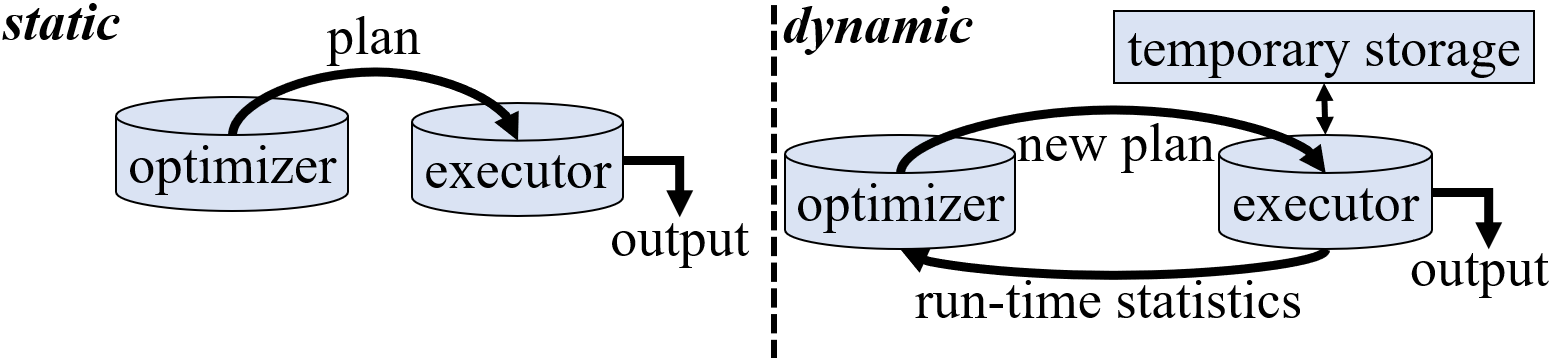
\includegraphics[width=\linewidth]{./pic/Figure1.png}
        \caption{Static and dynamic query optimization}
        \label{F1}
        \Description{In tradition structure, there is a unidirectional pipeline from optimizer to executor; and in breakup pipeline structure, there is a circle instead.}
    \end{figure}\par
    Re-optimization does not make drastic changes to the query execution engine. Instead, it detects during run-time whether the actual behavior of a query plan becomes significantly different from what was expected and attempts to correct the execution plan whenever it happens. In other words, re-optimization admits that the query optimizer can make mistakes in decisions and thus tries to alleviate them. In recent work, Perron et al. \cite{MichaelStonebraker} evaluated the performance of re-optimization on the Join Order Benchmark \cite{JOB}, and their result suggests that re-optimization can significantly reduce query execution time.\par
    Re-optimization makes use of the statistic of intermediate results, and in this paper, we refer to them as run-time statistics to distinguish them from statically collected statistics. By using run-time statistics, the optimizer improves cardinality estimation in two aspects: first, by replacing estimated statistics with run-time statistics, the optimizer reduces the cardinality estimation error caused by problematic assumptions. For example, the run-time statistics can include the actual distribution of attributes in the intermediate result, which leads to a more accurate cardinality estimation. Another aspect is that run-time statistics stop error propagation. The optimizer uses run-time statistics to replace the estimated cardinality, which essentially reduces the size of the join that needs to be estimated.\par
    Re-optimization can be classified as a specific case of the more general concept of adaptive query processing \cite{paper47}, in which query execution strategy changes adaptively based on the actual state during execution. Most existing adaptive query processing techniques keep the strict order between optimizer and executor. For example, parametric query optimization \cite{paper44} and Rio \cite{paper25} give the executor a set of possible optimal plans instead of giving one single plan. Thus, they can switch the plan during execution. Eddies \cite{paper30} generate a basic join tree by a simple pre-optimizer and can dynamically change the tuple pipeline in join operators during execution.

\subsection{Sub-plan Perspective} \label{S23}
\textcolor{blue}{
    We can summarize the general procedure of traditional re-optimization as follows:
    \begin{itemize}[leftmargin = 15pt]
        \item First, select a sub-tree of the global plan tree.
        \item Then, execute that sub-plan and materialize the result as a temporary table.
        \item Finally, replace the sub-tree with the table and re-optimize the remaining query.
    \end{itemize}
}\par
\textcolor{blue}{
    In traditional re-optimization, the materialized results are always the sub-trees of the global plan tree or so-called sub-plan. For example, in mid-query re-optimization \cite{Reopt}, the node whose subsequent operator is blocked (e.g., sort and hash) will be materialized. And in \textit{Pop} \cite{Pop}, the database system also materializes the sub-plans at the outer side of the nest-loop join. However, this sub-plan perspective has two problems.
}\par
\textcolor{blue}{
    First, re-optimization may be misled by the global plan if it deviates largely from the optimal one. Sub-plan perspective may choose a sub-plan that is the sub-tree of the global plan, but not the sub-tree of the optimal one. In that case, even if we re-optimize the remaining plan after executing the sub-plan, the join order still becomes sub-optimal. More seriously, as the problem scale of the remaining query is still large, the re-optimized plan can deviate significantly from the optimal plan again.
}\par
\textcolor{blue}{
    To illustrate how a bad global plan ruins re-optimization, we give the following example.
    \begin{Example}
        As shown in Figure \ref{F21}(a), due to an underestimation of cardinality, the global plan first decides to join relation $k$ and $mk$ by nest-loop join. However, in Figure \ref{F21}(b), the optimal choice is to join relation $ci$ and $n$ and then use the join result as a probe to index scan $k$ and $mk$. We assume a re-optimization happens immediately after the first join. Hence, the first sub-plan is $k \bowtie mk$, and we denote the materialized result as $S_1$. However, we still miss the opportunity to execute this query with the optimal execution plan. As shown in Figure \ref{F21}(c), the only way to correct back to the optimal plan is first to join $ci$ and $n$ in the re-optimized plan, but we cannot index scan $S_1$ as there is no index on the temporary relation. Instead, we have to use a hash join, which takes ten times more than index scan $k$ and $mk$.
    \end{Example}
}\par
    \begin{figure}[htb]
        \subfigure[\normalsize{Global plan}]
        {
            \begin{minipage}[t]{0.3\linewidth}
                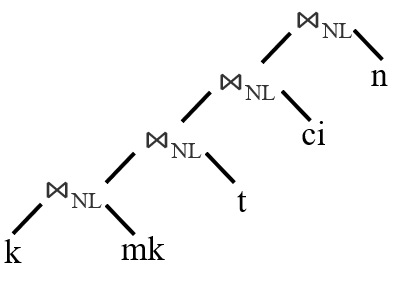
\includegraphics[width=\linewidth]{./pic/Figure21a.png}   
            \end{minipage}
        }
        \subfigure[\normalsize{Optimal plan}]
        {
            \begin{minipage}[t]{0.3\linewidth}
                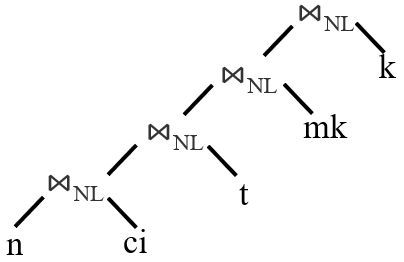
\includegraphics[width=\linewidth]{./pic/Figure21b.png}
            \end{minipage}
        }
        \subfigure[\normalsize{Re-Optimized plan after the first join}]
        {
            \begin{minipage}[t]{0.3\linewidth}
                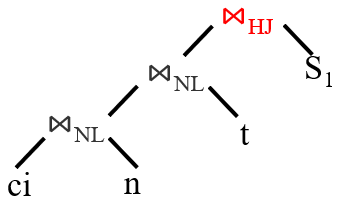
\includegraphics[width=\linewidth]{./pic/Figure21c.png}
            \end{minipage}
        }
        \centering
        \caption{Bad sub-plan example}
        \label{F21}
        \Description{}
    \end{figure}\par
\textcolor{blue}{
    And according to our observation, the phenomenon that the global plan hugely differs from the optimal one is not rare in the real world benchmark. Table \ref{T1} shows the ratio of queries whose global plans deviate hugely from the optimal plan in Join Order Benchmark. We will describe how to get the optimal plan in Section \ref{S5}. As shown in Figure \ref{F2}, we measure the similarity by the number of leaf nodes in the largest common sub-tree between the global plan and optimal plan: similarity is 0 means that the optimal plan is totally different from the global plan; 1 means they scan the same relation but do not join it with the same relation; and 2 means they execute the same first join, but their second joins are different.
}
    \begin{figure}[htb]
        \subfigure[\normalsize{Similarity is 0}]
        {
            \begin{minipage}[t]{0.3\linewidth}
                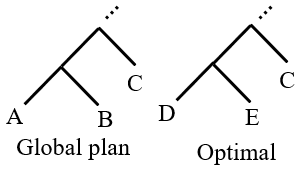
\includegraphics[width=\linewidth]{./pic/Figure2a.png}   
            \end{minipage}
        }
        \subfigure[\normalsize{Similarity is 1}]
        {
            \begin{minipage}[t]{0.3\linewidth}
                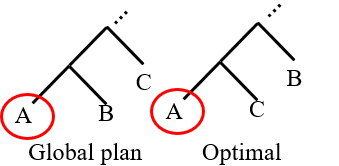
\includegraphics[width=\linewidth]{./pic/Figure2b.png}
            \end{minipage}
        }
        \subfigure[\normalsize{Similarity is 2}]
        {
            \begin{minipage}[t]{0.3\linewidth}
                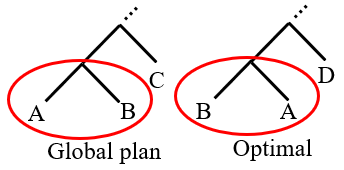
\includegraphics[width=\linewidth]{./pic/Figure2c.png}
            \end{minipage}
        }
        \centering
        \caption{The example of different similarity}
        \label{F2}
        \Description{}
    \end{figure}\par
\textcolor{blue}{
    From Table \ref{T1}, we can see that 13\% of the query plans completely deviate from the optimal plan, 12\% deviate from the optimal plan before the first join, and 32\% deviate from the optimal plan after the first join. In other words, no matter the size of the first sub-plan in sub-plan perspective, for 25\% queries in JOB, re-optimization will select the sub-optimal sub-plan at the beginning (similarity is 0 and 1). And suppose the first sub-plan has more than one join. In that case, re-optimization will choose a sub-optimal execution path for more than half queries (similarity is 0, 1 and 2).
}
    \begin{table}[htb]
        \caption{The ratio of queries whose global plans deviate hugely from the optimal plan}
        \label{T1}
        \begin{tabular}{c|c}
            \toprule
            Similarity & Ratio    \\
            \midrule
            0          & 13\%     \\
            1          & 12\%     \\
            2          & 32\%     \\
            > 2        & 43\%     \\
            \bottomrule
        \end{tabular}
    \end{table}\par
\textcolor{blue}{
    Second, for a given query, how often materialization will happen is unknown, which may incur a heavy overhead for materialization. In traditional re-optimizations, as we mentioned before, whether materialization happens depends on the type of plan nodes. We do not know whether and where the materialization will occur until the new plan becomes available. We call such a pattern the reactive pattern. The uncontrollability of materialization means non-robustness of the materialization overhead.
}\par
    
\subsection{Sub-query Perspective and Query Split Framework} \label{S24}
\textcolor{blue}{
    As the sub-plan perspective has the above problems, we propose a new perspective and reserve the general idea of changing the plan halfway through execution.
}\par
\textcolor{blue}{
    Different from materializing a sub-tree of the global plan (sub-plan), we split the query into sub-queries in advance and send them to the query processing engine as separate queries. Obviously, the global plan is discarded in this new perspective, and we call this perspective the \textit{sub-query perspective}.
}\par
\textcolor{blue}{
    Compared to the sub-plan perspective, our sub-query perspective has the following benefits:
    \begin{itemize}[leftmargin = 15pt]
        \item Do query optimization for each sub-query avoids the possible misleading of the global plan. Suppose a proper sub-query splitting strategy exists and a way to decide their execution orders (we will discuss them in Section \ref{S4}). In that case, the plan we get is more similar to the sub-tree of the optimal plan.
        \item As the size of each sub-query is small, according to Section \ref{S21}, the difficulty of query optimization decreases, and we can have more reliable execution plans for each sub-query.
        \item Because we split the query into sub-queries as soon as the query comes, we know exactly how often materialization will happen. Compared to the sub-plan perspective, our sub-query perspective is a proactive method. Thus, we ensure the robustness of the materialization overhead.
    \end{itemize}
}\par
    In this paper, we propose a new framework called \textit{query split} to cooperate with our sub-query perspective. In \textit{query split}, we execute a small part of the query each time and materialize its result until the entire query has been executed. Here we provide an example to demonstrate how \textit{query split} works in practice.
    \begin{Example}
        As shown in Figure \ref{F3}(a), we consider a query $G=R_1 \bowtie R_2 \bowtie R_3 \bowtie R_4 \bowtie R_5$ on five relations. First, we split query $G$ into three sub-queries, as shown in Figure \ref{F3}(b): $S_1=R_2 \bowtie R_3$, $S_2=R_3 \bowtie R_4 \bowtie R_5$, and $S_3=R_1 \bowtie R_2$. Then, we execute $S_1$ and materialize the result as temporary table $t_1$. Next, we replace $R_2$ and $R_3$ in $S_2$, $S_3$ by $t_1$, resulting in $S_2=t_1 \bowtie R_4 \bowtie R_5$, and $S_3=R_1 \bowtie t_1$, as shown in Figure \ref{F3}(c). Afterwards we execute the modified version of $S_2$, and materialize its result as $t_2$. Finally, as shown in Figure \ref{F3}(d), we replace $t_1$ in $S_3$ by $t_2$ to get $S_3=R_1 \bowtie t_2$, and then replan and execute it to obtain the result.
    \end{Example}
    \begin{figure}[htb]
        \subfigure[\normalsize{Join Graph of $G$}]
        {
            \begin{minipage}[t]{0.47\linewidth}
                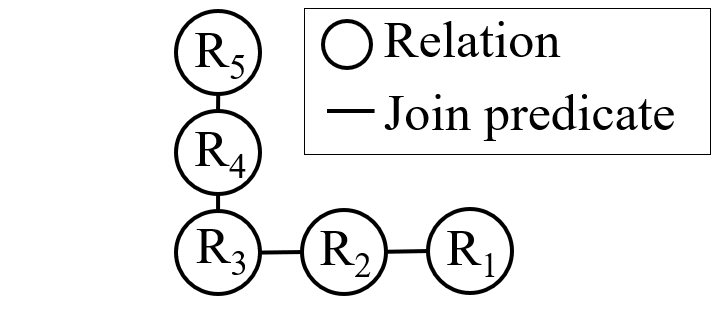
\includegraphics[width=\linewidth]{./pic/Figure3a.png}   
            \end{minipage}
        }
        \subfigure[\normalsize{$G$ with sub-queries $S_1$, $S_2$, $S_3$}]
        {
            \begin{minipage}[t]{0.47\linewidth}
                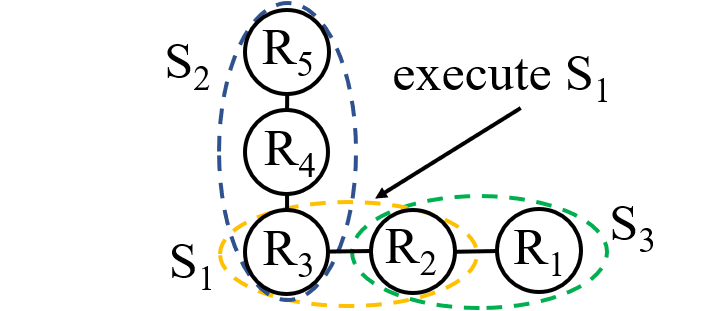
\includegraphics[width=\linewidth]{./pic/Figure3b.png}
            \end{minipage}
        }
        \subfigure[\normalsize{$G$ after executing $S_1$}]
        {
            \begin{minipage}[t]{0.47\linewidth}
                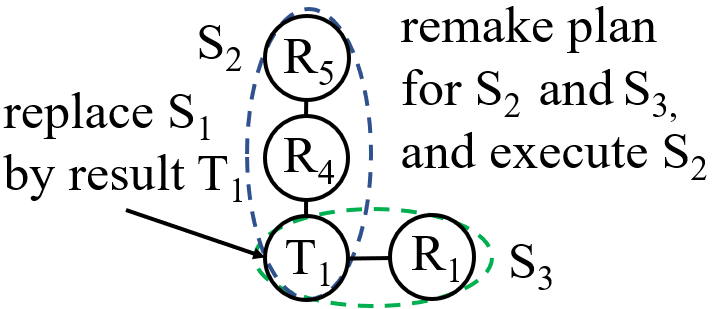
\includegraphics[width=\linewidth]{./pic/Figure3c.png}
            \end{minipage}
        }
        \subfigure[\normalsize{$G$ after executing $S_1$ and $S_2$}]
        {
            \begin{minipage}[t]{0.47\linewidth}
                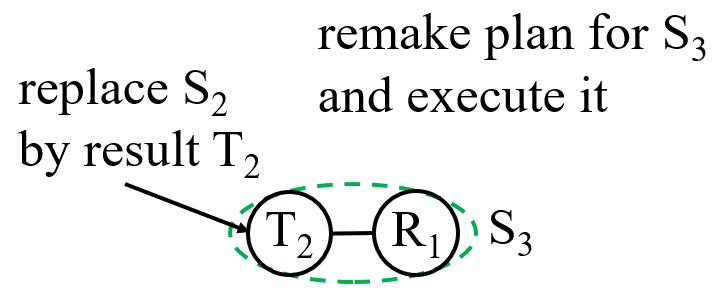
\includegraphics[width=\linewidth]{./pic/Figure3d.png}
            \end{minipage}
        }
        \centering
        \caption{\textit{query split} example}
        \label{F3}
        \Description{}
    \end{figure}\par
    More generally, \textit{query split} works as follows. First, for a given query, we split it into several small sub-queries by a sub-query splitting procedure. Then we compute the result of the original query using these sub-queries:
    \begin{itemize}[leftmargin = 15pt]
        \item Each time, choose a sub-query to execute and then remove it from the set of sub-queries.
        \item After running a sub-query $q_i$ and collecting run-time statistics, modify other sub-queries and remake their execution plans.
        \item When no sub-query is left, merge some sub-queries results to obtain the original query result.
    \end{itemize}\par
\textcolor{blue}{
    \textit{Query split} framework has two characteristics:
    \begin{itemize}[leftmargin = 15pt]
        \item Traditional re-optimization techniques determine the sub-query (sub-plan) to be executed after query optimization. In contrast, query split determines what sub-queries will be executed before the query optimization stage.
        \item \textit{Query split} can also implement the re-optimization with the sub-plan perspective by designing a specific splitting algorithm. We use the global plan as an input for the query splitting algorithm, and every time a sub-query is executed, we do query splitting again.
    \end{itemize}
}\par
    \textit{Query split} is a new attempt at re-optimization, and we hope to use this work to draw more attention and research to this direction. Our new framework opens a fresh perspective to the query optimization problem. As shown in Section \ref{S5}, \textit{query split} outperforms the built-in PostgreSQL optimizer by a large margin and reaches near-optimal execution time in the Join Order Benchmark.

\section{Formulation \& Definition} \label{S3}
    In this section, we formalize \textit{query split}. We first define the concept of select-projection-join query and formally describe \textit{query split} for such queries (in Section \ref{S31}). Then, we design an implementation for reconstruction algorithm, which is one of the components of \textit{query split}, and prove its correctness (in Section \ref{S32}).
\subsection{Framework Overview} \label{S31}
    In this section, we give an overview of \textit{query split} framework. For simplicity, we temporarily restrict our attention to select-projection-join (SPJ) queries in the following three sections, which only involve select, projection, and join operators. These three operators are chosen because they can be connected together to compose most of the basic SQL SELECT queries, covering all the queries in the Join Order Benchmark \cite{JOB}. \textit{Query split} can be extended to handle more general queries, which is discussed in Section \ref{S6}.\par
    First, let us define a normal form of SPJ queries. Then by relational algebra manipulation, every SPJ queries can be transformed into the following normal form, in which we denote by \textbf{\textit{R}} a set of relations, \textbf{\textit{S}} a set of select predicates over \textbf{\textit{R}} and \textbf{\textit{P}} a set of projection attributes, via equivalence rules (details can be found in Appendix A).
    $$q(\textbf{\textit{R}},\textbf{\textit{S}},\textbf{\textit{P}})=\Pi_{\textbf{{\textit{P}}}}(\sigma_{\textbf{\textit{S}}}(r_1 \times r_2 \times... \times r_m)),r_i \in \textbf{\textit{R}}$$
    Now, we can formally describe \textit{query split}. The framework consists of five components: query splitting algorithm, run-time statistics collector, query optimizer, query executor, and the reconstruction algorithm. The relationship between five components are shown in Figure \ref{F4}. Query splitting algorithm takes the global query as input and splits it into sub-queries, and then we obtain the result via the following steps:
    \begin{enumerate}[leftmargin = 15pt]
        \item In each iteration, the reconstruction algorithm picks a sub-query and sends it to the query optimizer.
        \item The query optimizer makes an execution plan and delivers it to the query executor.
        \item The query executor executes the plan, materialize the results and sends them to statistic collector.
        \item The run-time statistic collector obtains new statistics, which can help the optimizer make better plans for the remaining sub-queries in the following iterations.
        \item After all subqueries have been executed, the reconstruction algorithm reconstructs the final query result relation from sub-query results.
    \end{enumerate}
    \begin{figure}[htb]
        \centering
        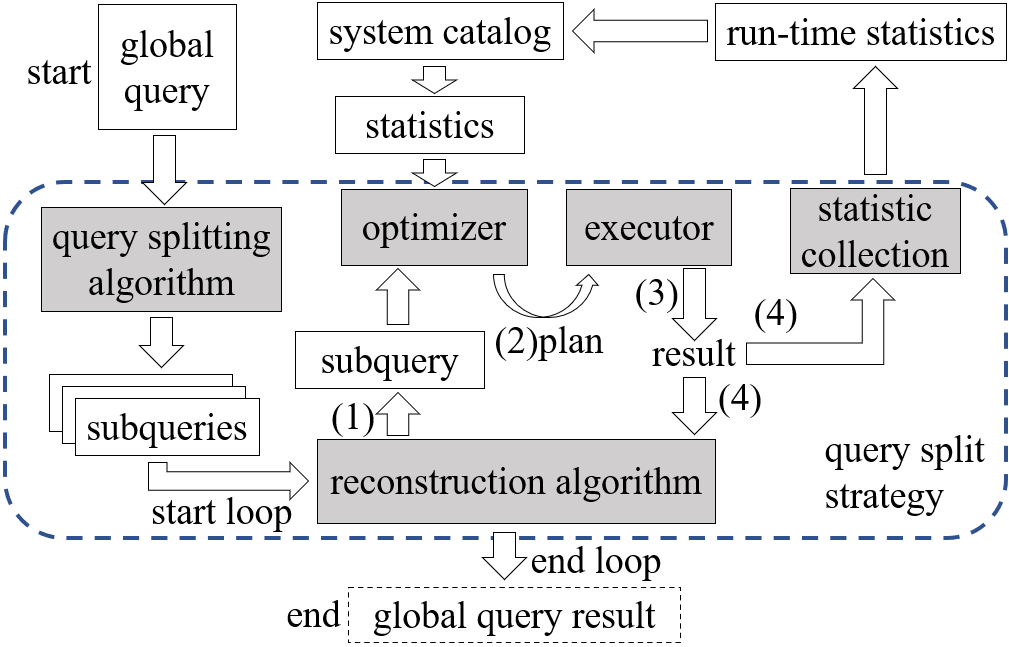
\includegraphics[width=\linewidth]{./pic/Figure4.png}
        \caption{The framework of \textit{query split}}
        \label{F4}
        \Description{}
    \end{figure}\par
    Note that statistics collector, query optimizer, and query executor are existing components in RDBMS. In the following, we define query splitting algorithm and reconstruction algorithm, the two new concepts that we propose in this paper.\par
    We first formalize the concept of sub-query and query splitting algorithm, in which we stipulate that sub-queries do not contain projection operations. The definition of query splitting algorithm here is abstract, and we will discuss possible concrete implementations in Section 4.1.
    \begin{Definition} \label{D1}
        Given two $SPJ$ queries q(\textbf{\textit{R}}, \textbf{\textit{S}}, \textbf{\textit{P}}) and q$'($\textbf{\textit{R}}$',$\textbf{\textit{S}}$')$. If \textbf{\textit{R}}$'\subseteq$\textbf{\textit{R}} and \textbf{\textit{S}}$'\subseteq$\textbf{\textit{S}}, then q$'$ is said to be a sub-query of query q. Query splitting algorithm is an algorithm which takes a SP$J$ query q as input and returns a set of sub-queries of q.
    \end{Definition}\par
    Next, we define the concept of reconstruction algorithm.\par
    \begin{Definition} \label{D2}
        Reconstruction algorithm is an algorithm that takes a set of sub-queries \textbf{\textit{Q}} and a set of projection attributes \textbf{\textit{P}} as input and returns a reconstructed relation. A reconstruction algorithm A is correct with respect to a query splitting algorithm B if, for every SP$J$ query q(\textbf{\textit{R}}, \textbf{\textit{S}}, \textbf{\textit{P}}), the reconstructed relation is always equal to the result of the original query, if we feed the output of B on q together with \textbf{\textit{P}} as input of A.
    \end{Definition}\par
    Clearly, not every query splitting algorithm has a corresponding reconstruction algorithm. A crucial question here is under which conditions a correct reconstruction algorithm exists. To answer this question, we define the concept of subquery cover.
    \begin{Definition} \label{D3}
        Given a SP$J$ query q(\textbf{\textit{R}}, \textbf{\textit{S}}, \textbf{\textit{P}}), let \textbf{\textit{Q}}=$\{q_1(\textbf{\textit{R}}_1,\textbf{\textit{S}}_1)$, ..., $q_n(\textbf{\textit{R}}_n,\textbf{\textit{S}}_n)\}$ be a set of subqueries of q. We denoted R(\textbf{\textit{Q}})=$\cup_{i=1}^n \textbf{\textit{R}}_i$ and S(\textbf{\textit{Q}})=$\cup_{i=1}^n \textbf{\textit{S}}_i$. \textbf{\textit{Q}} is said to cover $q$ (\textbf{\textit{Q}}$\rightharpoonup_c$q) if,\par
        (1) R(\textbf{\textit{Q}})=\textbf{\textit{R}}\par
        (2) S(\textbf{\textit{Q}}) logically implies \textbf{\textit{S}}. \footnote[1]{``A logically implies B" means that each predicate from B can be inferred by A.}
    \end{Definition}\par
    Intuitively, the reconstruction can succeed only if there is no information loss between the set of sub-queries and the original query, and the sub-query cover concept formalizes this intuition. To ensure a correct reconstruction algorithm exist, the set of sub-queries \textbf{\textit{Q}} returned by a query splitting algorithm with query q needs to satisfy \textbf{\textit{Q}}$\rightharpoonup_c$q. And we give a simple reconstruction algorithm that guarantees correctness under such conditions in the following section.

\subsection{Replacement Reconstruction} \label{S32}
    In this section, we propose a concrete reconstruction algorithm called \textit{replacement reconstruction}, which is correct with respect to every query splitting algorithm that are guaranteed to cover the original query. The correctness of this algorithm will be proved later.
    \begin{figure}[htb]
        \centering
        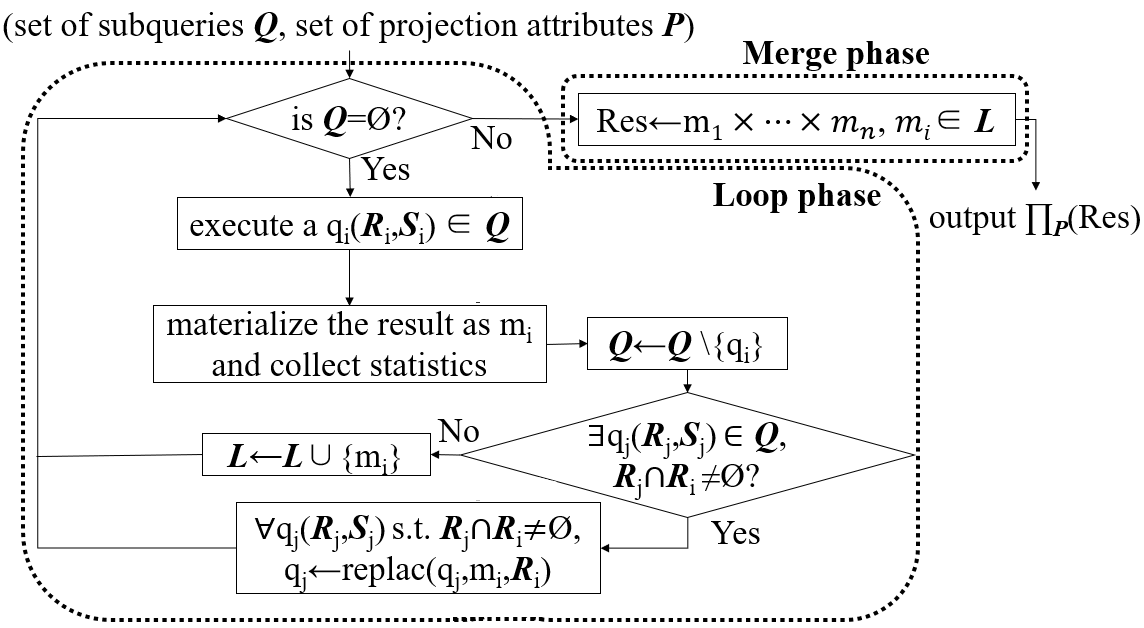
\includegraphics[width=\linewidth]{./pic/Figure5.png}
        \caption{Replacement reconstruction}
        \label{F5}
        \Description{}
    \end{figure}\par
    Figure \ref{F5} shows a flow chart that explains how \textit{replacement reconstruction} algorithm works. The algorithm takes the set of sub-queries \textbf{\textit{Q}} and the set of projection attributes \textbf{\textit{P}} as inputs, and use the following steps to reconstruct the query result.
    \begin{algorithm}[htb]
        \caption{Replacement Reconstruction}
        \begin{algorithmic}[1]
            \Require \textbf{\textit{Q}} a set of sub-queries, \textbf{\textit{P}} a set of projection attributes
            \Function{ReplacRecon}{\textbf{\textit{Q}}, \textbf{\textit{P}}}
                \State \textbf{\textit{L}} $\gets \emptyset$
                \While{\textbf{\textit{Q}} $\neq \emptyset$}
                    \State $\backslash$* use QSELECT() to choose a sub-query from \textbf{\textit{Q}} *$\backslash$
                    \State $q_i(\textbf{\textit{R}}_i,\textbf{\textit{S}}_i) \gets$ \Call{QSELECT}{\textbf{\textit{Q}}}
                    \State $\backslash$* EXEC() executes sub-query and materialize results *$\backslash$
                    \State $m_i \gets$ \Call{EXEC}{$q_i$}
                    \State $\backslash$* STAT() collects the run-time statistics*$\backslash$
                    \State $system\_catalog \gets$ \Call{STAT}{$m_i$}
                    \State \textbf{\textit{Q}} $\gets$ \textbf{\textit{Q}} $\setminus \{q_i\}$
                    \State $flag \gets 0$
                    \For{$q_j(\textbf{\textit{R}}_j,\textbf{\textit{S}}_j) \in$ \textbf{\textit{Q}}}
                        \If{$\textbf{\textit{R}}_j \cap \textbf{\textit{R}}_i \neq \emptyset$}
                            \State $\backslash$* replace subset $\textbf{\textit{R}}_j \cap \textbf{\textit{R}}_i$ in $\textbf{\textit{R}}_j$ with $m_i$ *$\backslash$
                            \State $q_j \gets$ replac($q_j$, $m_i$, $\textbf{\textit{R}}_i$)
                            \State $flag \gets 1$
                        \EndIf
                    \EndFor
                    \If{$flag=0$}
                        \State \textbf{\textit{L}} $\gets$ \textbf{\textit{L}} $\cup \{m_i\}$
                    \EndIf
                \EndWhile
                \State $Res \gets m_1 \times m_2 \times ... \times m_n, m_i \in$ \textbf{\textit{L}}
                \State \Return{$\Pi_{\textbf{\textit{P}}}(Res)$}
            \EndFunction
        \end{algorithmic}
    \end{algorithm}
    \begin{itemize}[leftmargin = 15pt]
        \item \textbf{Initial}: initialize the set of sub-query results \textbf{\textit{L}} as empty set.
        \item \textbf{Loop(execute)}: execute a sub-query $q_i(\textbf{\textit{R}}_i,\textbf{\textit{S}}_i)$ from \textbf{\textit{Q}} and materialize the result as $m_i$, then collect run-time statistics. 
        \item \textbf{Loop(modify)}: remove $q_i(\textbf{\textit{R}}_i,\textbf{\textit{S}}_i)$ from \textbf{\textit{Q}}, then pick out all sub-queries $q_j(\textbf{\textit{R}}_j,\textbf{\textit{S}}_j)$ whose set of relations $\textbf{\textit{R}}_j$ intersects with $\textbf{\textit{R}}_i$, modify these sub-queries via a specific protocol that will be described later $q_j \gets$ replac$(q_j, m_i, \textbf{\textit{R}}_i)$. If there is no such $q_j$, add $m_i$ to \textbf{\textit{L}}. After this, check whether \textbf{\textit{Q}} is empty and repeat the loop if not.
        \item \textbf{Merge}: when \textbf{\textit{Q}} is empty, compute the Cartesian product of all relations in \textbf{\textit{L}} and project on the result by \textbf{\textit{P}}, and the end result is the reconstructed relation.
    \end{itemize}\par
    It remains to describe how replac$(q_j, m_i, \textbf{\textit{R}}_i)$ works. It actually modifies the sub-query $q_j(\textbf{\textit{R}}_j,\textbf{\textit{S}}_j)$ from two aspects.
    \begin{itemize}[leftmargin = 15pt]
        \item First, replace all relations in $\textbf{\textit{R}}_i \cap \textbf{\textit{R}}_j$ by $m_i$. In other words, set the set of relations of $q_j$ as $\textbf{\textit{R}}_j \gets \textbf{\textit{R}}_j \setminus \textbf{\textit{R}}_i \cup \{m_i\}$.
        \item After replacing old relations from $\textbf{\textit{R}}_j$ with $m_i$, some predicates in $\textbf{\textit{S}}_j$ would be referencing removed relations. Update those predicates by using the corresponding attributes in $m_i$ instead.
    \end{itemize}\par
    Now we can prove the correctness of replacement reconstruction algorithm.
    \begin{Theorem}[1] \label{Th1}
        Let q(\textbf{\textit{R}}, \textbf{\textit{S}}, \textbf{\textit{P}}) be an SP$J$ query, \textbf{\textit{Q}} be a set of sub-queries of q. If \textbf{\textit{Q}}$\rightharpoonup_c$q, then the output of the replacement reconstruction algorithm is equal to the result of q.
    \end{Theorem}\par
    This implies that the replacement reconstruction algorithm is a correct reconstruction algorithm for any query splitting algorithm that guarantees its output to cover the original query. The proof of this theorem can be found in Appendix B.\vspace{6pt}\\
    \textit{Remark}: In Definition \ref{D1}, we assume that there is no projection operation in sub-queries for simplicity. In practice, we can push down the projection operation to each sub-query to effectively reduce the size of the temporary relation and minimize execution time. In principle, any attribute which doesn't appear in other sub-queries can be safely projected away.

\section{Detail Implementation} \label{S4}
    Although we formally described the \textit{query split} in Section \ref{S3}, there are still some relatively flexible components. In this section, we examine these components in more detail, and provide some concrete implementations: the query splitting algorithm (in Section \ref{S41}) and the criterion for selecting which sub-query to execute each time (in Section \ref{S42}). However, since our paper aims to verify the general effectiveness of \textit{query split}, an in-depth research of these components is beyond the scope of this paper. The contents of this section only serve as some preliminary designs for reference.
\subsection{Query Splitting Algorithm} \label{S41}
\textcolor{blue}{
    In this section, we propose our query splitting algorithm \textit{RelationshipCenter}, and two other algorithms (\textit{MinSubquery} and \textit{EntityCenter}) for later experimental contrast.
}
    \subsubsection{RelationshipCenter} \label{S412}
        Because \textit{query split} needs to materialize the result of sub-queries, it would be beneficial to attempt to constrain the size of sub-query results when constructing the sub-queries. There are several potential benefits for doing this: first, a small sub-query result can speed up the later execution, as the completed sub-queries will often be used in other sub-queries. Another benefit is that it improves the framework's robustness by using less memory. In \textit{query split}, each sub-query result must be materialized in memory after execution, and hence sub-queries with bounded result sizes lead to more stable memory usage.\par
\textcolor{blue}{
        According to Axel et al. \cite{USE}, if all the operators in a query are non-expanding operators, the result size of the query is constrained. The non-expanding operator is a kind of operator whose result size does not exceed the input size. For example, primary-foreign-key join ensures the join result will not exceed the relation that contains the foreign key. Besides, filter operation also belongs to the non-expanding operator. According to the property of non-expanding operators, we can constrain the result size of sub-queries. Suppose each join in a sub-query is the primary-foreign-key join and all foreign keys locate in the same relation. In that case, the size of the sub-query result will not exceed the size of that relation.
}\par
        To ensure the above conditions, we first introduce two new concepts: entity relation and relationship relation, which are inspired by the entity-relationship diagram \cite{paper32}. If the primary key of a relation is referenced by another relation as foreign key, we denote such relation as an entity relation. For relations that do not have a primary key or their primary keys are not referenced by any other relation, we denote them as relationship relations.\par
\textcolor{blue}{
        With the above definitions, we can see that when a sub-query consists of a relationship relation with several entity relations, each join in this sub-query is the primary-foreign-key join, and thus the cardinality of the sub-query result will not exceed the size of the relationship relation. Based on this, we propose the \textit{RelationshipCenter} algorithm to control the size of each sub-query. The algorithm ensures that most sub-queries contain one relationship and multiple entity relations. The concrete steps of \textit{RelationshipCenter} are shown as follows.
}
        \begin{itemize}[leftmargin = 15pt]
            \item First, we classify all relations into two types: relationship and entity by the above definitions.
            \item Next, we remove redundant select predicates, and we prefer to reserve foreign-key joins as much as possible.
            \item Then, we construct a directed graph for the given query, in which each vertex represents a relation. For each foreign-key join predicate, we create an edge from the relation which contains the foreign key to the relation where primary key comes. For every other select predicate that spans multiple relations, we consider all possible pairs from the involved relations, and create one or two edges between them, depending on their relation types: if both relations are the same type, we create two edges in both directions. Otherwise, we create an edge from relationship relation to entity relation.
            \item Last, for each relation that connects to other relations, we create a sub-query based on this relation. The relation set of the sub-query contains the given relation and all relations it links to. The select predicate set contains all predicates over the relation set.
        \end{itemize}\par
        Example \ref{E4} demonstrates how \textit{RelationshipCenter} works.
        \begin{figure}[htb]
            \subfigure[\normalsize{Global query}]
            {
                \begin{minipage}[t]{0.47\linewidth}
                    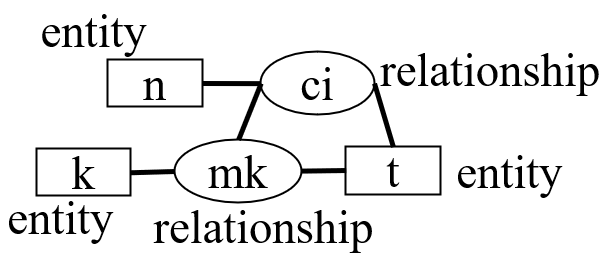
\includegraphics[width=\linewidth]{./pic/Figure6a.png}
                \end{minipage}
            }
            \subfigure[\normalsize{Sub-queries}]
            {
                \begin{minipage}[t]{0.47\linewidth}
                    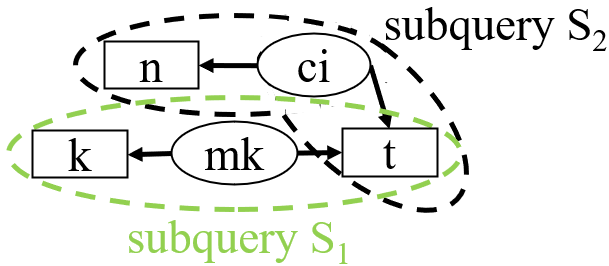
\includegraphics[width=\linewidth]{./pic/Figure6b.png}
                \end{minipage}
            }
            \centering
            \caption{Join graph split by \textit{RelationshipCenter}}
            \label{F6}
            \Description{}
        \end{figure}
        \begin{Example}[RelationshipCenter] \label{E4}
            As shown in Figure \ref{F6}(a), the query consists of one non-foreign key join ($mk \bowtie ci$) and four foreign key joins ($k \bowtie mk$, $t \bowtie mk$, $t \bowtie ci$ and $n \bowtie ci$). Hence, relation $mk$ and $ci$ are relationships and relation $k$, $n$, $t$ are entities. Then as shown in Figure \ref{F6}(b), we first remove $mk \bowtie ci$ because it is redundant, then draw a directed graph with four edges ($E_1=mk \rightarrow k$, $E_2=mk \rightarrow t$, $E_3=ci \rightarrow t$ and $E_4=ci \rightarrow n$), corresponding to join predicates. Next, consider all relations: relation $k$, $n$ and $t$ don't connect to any other relation, hence we do not create sub-queries for them; relation $mk$ connects to $k$ and $t$, resulting in sub-query $S_1=\sigma_{f_k}(k) \bowtie mk \bowtie \sigma_{f_t}(t)$; relation $ci$ connects to $n$ and $t$, and we have sub-query $S_2=\sigma_{f_n}(n) \bowtie ci \bowtie \sigma_{f_t}(t)$.
        \end{Example}\par
        Then, to illustrate that the query splitting algorithm is essential for the performance, we propose two other algorithms (\textit{MinSubquery} and \textit{EntityCenter}) for contrast and compare them with \textit{RelationshipCenter} in Section \ref{S5}.

    \subsubsection{MinSubquery} \label{S411}
        This is the most straightforward query splitting algorithm, in which we split the query into minimal sub-queries. For each select predicate that spans more than one relation, we use those relations to construct a relation set $\textbf{\textit{R}}_i$. Then we construct the set of select predicates $\textbf{\textit{S}}_i$ to contain all the select predicates over $\textbf{\textit{R}}_i$. We use an example query (shown in Figure \ref{F19}(a)) to demonstrate the procedure of \textit{MinSubquery} below.
        \begin{Example}[MinSubquery] \label{E3}
            As shown in Figure \ref{F7}(a), there are five join predicates (denoted by $k \bowtie mk$, $mk \bowtie ci$, $n \bowtie ci$, $t \bowtie mk$ and $t \bowtie ci$) and three select predicates over relation $k$, $n$, and $t$ (denoted by $f_k$, $f_n$ and $f_t$). To create sub-queries, first construct the following relation sets involved in join predicates: $\textbf{\textit{R}}_1=\{k,mk\}$, $\textbf{\textit{R}}_2=\{ci,mk\}$, $\textbf{\textit{R}}_3=\{ci,n\}$, $\textbf{\textit{R}}_4=\{mk,t\}$, $\textbf{\textit{R}}_5=\{ci,t\}$. Then, for each relation set $\textbf{\textit{R}}_i$, $\textbf{\textit{S}}_i$ is equal to the union of all select predicates in the original query over $\textbf{\textit{R}}_i$. As shown in Figure \ref{F7}(b), this results in five sub-queries $q_1=\sigma_{f_k}(k) \bowtie mk$, $q_2=mk \bowtie ci$, $q_3=\sigma_{f_n}(n) \bowtie ci$, $q_4=\sigma_{f_t}(t) \bowtie mk$ and $q_5=ci \bowtie \sigma_{f_t}(t)$.
        \end{Example}
        \begin{figure}[htb]
            \subfigure[\normalsize{The example query}]
            {
                \begin{minipage}[t]{0.47\linewidth}
                    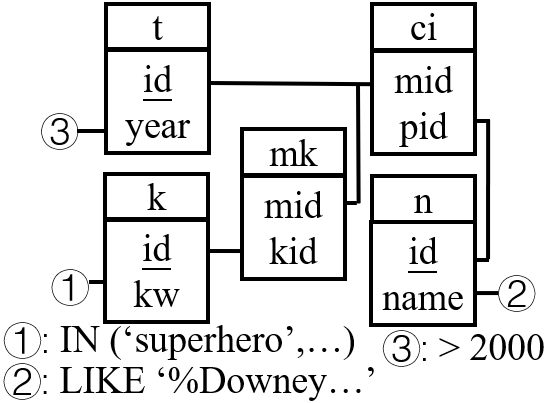
\includegraphics[width=\linewidth]{./pic/Figure7a.png}
                \end{minipage}
            }
            \subfigure[\normalsize{Sub-queries}]
            {
                \begin{minipage}[t]{0.47\linewidth}
                    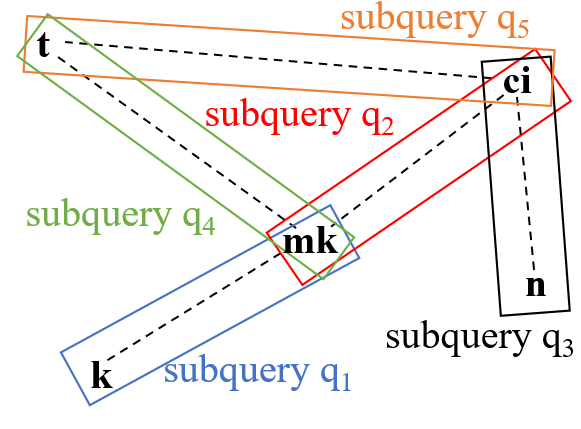
\includegraphics[width=\linewidth]{./pic/Figure7b.png}
                \end{minipage}
            }
            \centering
            \caption{Join graph split by \textit{MinSubquery}}
            \label{F7}
            \Description{}
        \end{figure}
    
    
    \subsubsection{EntityCenter} \label{S413}
        If we reverse the direction of edges in the directed graph in \textit{RelationshipCenter}, we can get another query splitting algorithm. In this algorithm, the centers of sub-queries are entity relations, and we name this algorithm \textit{EntityCenter}.
    
\subsection{Execution Order Decision} \label{S42}
    In this section, we propose some feasible criteria to decide which sub-query to execute each time. Although we have proved that execution order does not affect the correctness of \textit{query split}, different execution orders can lead to different execution time. Therefore, we give some feasible implementations as the candidates and evaluate their efficiency in Section \ref{S5}.
    \subsubsection{Heuristic-based Algorithm} \label{S421}
\textcolor{blue}{
    We propose a heuristic rule to order the sub-queries based on the \textit{ranking function}. We first take the execution plans of the sub-query as input and assign a numeric value to each by \textit{ranking function}. Then, we choose the sub-query with the lowest numeric value each time and return this sub-query and its execution plan to execute.
}\par
\textcolor{blue}{
    To build the ranking function, we need to consider what parameters we can get from a given plan and which are suitable inputs for ranking functions. For a given plan, we can get the cost estimation of that plan and its cardinality estimation. Intuitively, the cost of a plan indicates the current benefit of the plan. And the cardinality of the result represents the future benefit of the plan, since a small intermediate result will speed up the future sub-queries. Thus, we take both cost estimation and row estimation of the sub-query as candidate inputs for ranking functions.
}\par
    We have designed some ranking functions for the algorithm in Table \ref{T2}. We denote $q$ a sub-query and $plan(q)$ the execution plan made by optimizer, $plan(q).cost$ the estimated cost of $plan(q)$, and $row(q)$ the estimated size of its result. The most basic approach is to use only cost or row of sub-queries for ranking ($cost(q)$ and $row(q)$). However, these approaches fail to consider the future influence or the current benefit. Take both into consideration, we designed other three candidates $row\_hybrid(q)$, $hybrid\_sqrt(q)$ and $hybrid\_log(q)$ with detailed expression in Table \ref{T2}.
    \begin{table}[htb]
        \caption{The expression of different ranking functions}
        \label{T2}
        \begin{tabular}{c|c}
            \toprule
            ranking function  & expression                   \\
            \midrule
            $cost(q)$         & $plan(q).cost$               \\
            $row(q)$          & $row(q)$                     \\
            $row\_hybrid(q)$  & $plan(q).cost*row(q)$        \\
            $hybrid\_sqrt(q)$ & $plan(q).cost*\sqrt{row(q)}$ \\
            $hybrid\_log(q)$  & $plan(q).cost*\log(row(q))$  \\
            \bottomrule
        \end{tabular}
    \end{table}  
        
    \subsubsection{Global Plan-based Algorithm} \label{S422}
\textcolor{blue}{
    The order decision algorithms we introduce above are based on the sub-query perspective, which totally discards the global plan. In contrast, we propose an algorithm called \textit{global\_sel} that chooses which sub-query to execute according to the global plan.
}\par
    \textit{Global\_sel} starts the selection process with the global plan generated from the original query. Then, given an execution tree for the original query, we choose the deepest operator node, find the relations involved in the operator, and select the sub-query whose relation set contains those relations. If multiple sub-queries can be selected, we choose one of them by an arbitrary tie-breaking rule.
    \begin{figure}[htb]  
        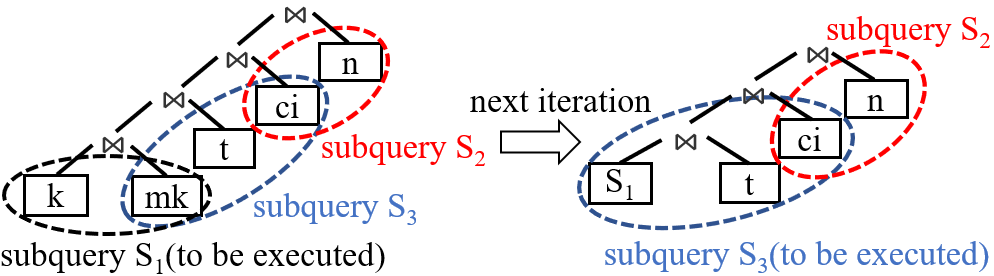
\includegraphics[width=\linewidth]{./pic/Figure8.png}
        \centering
        \caption{The illustration of \textit{global\_sel}}
        \label{F8}
        \Description{}
    \end{figure}\par
    Example \ref{E5} illustrates the procedure for the global plan-based algorithm.
    \begin{Example}[Global\_sel] \label{E5}
        We split the query into three subqueries $S_1=\sigma_{f_k}(k) \bowtie mk$, $S_2=\sigma_{f_n}(n) \bowtie ci$, and $S_3=ci \bowtie \sigma_{f_t}(t) \bowtie mk$. As shown in Figure \ref{F8}, at the beginning, the deepest non-leaf node in global plan is $k \bowtie mk$, and the involved relations are $\{k,mk\}$. Hence, sub-query $S_1$ would be first executed because it is the only sub-query whose relation set contains $k$ and $mk$. Then we materialize the sub-query result as a temporary table, and call optimizer for the remainder of the original query. In this iteration, the deepest non-leaf node in modified global plan is $S_1 \bowtie t$, so we choose $S_3$ because its relation set contains $S_1$ and $t$.
    \end{Example}

\section{Experiment} \label{S5}
    \textcolor{blue}{
    As we have motivated \textit{query split} and introduced all the details, we evaluate its performance on real-world workload in this section. We first describe how our experiments are organized (Section \ref{S51}). Next, we evaluate the performance impact of different query splitting algorithms and execution order decisions (Section \ref{S52}). Then, we investigate the sensitivity of heuristic-based order algorithms for the accuracy of cardinality estimation (Section \ref{S53}). And we compare a fine-tuned \textit{query split} implementation with baselines (Section \ref{S54}). We also discuss the materialization overhead among re-optimization techniques (Section \ref{S55}). Last, we discuss the influence of collecting different run-time statistics (Section \ref{S56}).
}
\subsection{Experiment Setup} \label{S51}
\textcolor{blue}{
    Our experiments are performed on a 64-bit Windows 10 computer with an Intel Core i9-10900K CPU (3.70 GHz) and 128GB RAM. We use the source code of PostgreSQL 12.3 as the basis for our implementations. In PostgreSQL, ”analyze” is the command that manually orders the optimizer to collect statistics for base relations. We call the same routine to gather the run-time statistics. In addition, we set max parallel workers to 0, so the CPU only uses one core during query processing. Furthermore, we increase the effective cache size to 8GB, and other parameters are set as default.
}\par
    We use Join Order Benchmark (JOB) \cite{JOB} as our experiment workload. JOB is a real-world workload over the IMDB dataset and has a high value for evaluating the performance of RDBMS. JOB has 113 queries, and 91 of them have non-empty results. We run these 91 queries and record their latency as reported by PostgreSQL.\par
    We have released the source code of \textit{query split} that we used in experiments on Github. \footnote[2]{https://github.com/zhaojy20/break-up-pipeline.}

\subsection{Different Implementations of sub-query perspective} \label{S52}
\textcolor{blue}{   
    We first evaluate the performance of different implementations of \textit{query split}. We test the total end-to-end latency for different sub-query splitting algorithms with all execution order decision strategies, and the result is shown in Table \ref{T3}. There are B+ tree indexes on both primary and foreign key attributes.
}
    \begin{table*}[htb]
        \caption{Total latencies for different implementations on JOB}
        \label{T3}
        \begin{tabular}{c|ccc}
            \toprule
            \diagbox{Function}{Latency(s)}{Strategy} & \textit{RelationshipCenter} & \textit{MinSubquery} &  \textit{EntityCenter} \\
            \midrule
            $cost(q)$                                &              421            &          463         &            378         \\
            $row(q)$                                 &              348            &          474         &            407         \\         
            $row\_hybrid(q)$                         &              295            &          427         &            350         \\
            $hybrid\_sqrt(q)$                        &              328            &          418         &            339         \\
            $hybrid\_log(q)$                         &              327            &          428         &            349         \\
            $global\_sel$                            &              356            &          401         &            413         \\
            \bottomrule
        \end{tabular}
    \end{table*}\par
    From Table \ref{T3}, we can conclude that both query splitting algorithms and execution order decisions influence the end-to-end latency. \textit{Minsubquery} uses the longest time for every execution order among query splitting algorithms. This result may be due to too much materialization, which apparently slows down the execution speed. The result suggests that \textit{Minsubquery} is not a good choice for query splitting. In most cases, \textit{RelationshipCenter} has the lowest latency, which proves our proposal that constraining the sub-query size can benefit the query execution latency.\par
\textcolor{blue}{
    Next, we observe that the end-to-end latency between five execution order decisions also changes significantly. $row(q)$, $cost(q)$, and $hybrid\_log(q)$ are the worst sub-query order selection strategies, as there is a gap between the weights given on row and cost. On the other hand, $hybrid\_sqrt(q)$ and $row\_hybrid(q)$ perform pretty closely. This finding indicates that the concrete parameters are unimportant as long as we consider current and future benefits with similar weights.
}\par
\textcolor{blue}{
    Meanwhile, although $global\_sel$ provides a global view, it does not outperform the heuristic rule based methods. Actually, the performance of $global\_sel$ is worse than heuristic rule based methods for most query splitting algorithms. This result proves our statement that the global plan may mislead the re-optimization. As a result, the execution order based on the global plan performs poorly.
}\par

\subsection{Sensitivity of Order Algorithm for CE Accuracy} \label{S53}
\textcolor{blue}{
    As our ranking functions take cardinality as an input, they may be sensitive to the accuracy of cardinality estimation. Therefore, we do the following experiments to investigate how the cardinality estimation error influences heuristic-based execution order decision algorithms.
}\par
\textcolor{blue}{
    The first step of this experiment is to get the accurate cardinality of every intermediate join result and the execution plan based on it. To this end, we make an optimal optimizer by following methods. We first execute all the possible sub-expression of the given query in advance and record their accurate cardinality. And then, we inject these actual values into the PostgreSQL optimizer by the method proposed by Cai, Balazinska, and Suciu \cite{PessimisticCE}. Thus, the optimizer knows the actual size of each intermediate relation and can make the optimal plan.
}\par
\textcolor{blue}{
    Then, we add noise to the accurate cardinality in order to get the cardinality with the artificial error. The formula for adding error is shown below, where $G(m, n)$ is a Gaussian distribution with mean $m$ and standard error $n$.
}
    $$ est\_card = 2^{G(m, n)} * true\_card $$\par
\textcolor{blue}{
    The total end-to-end latency of different execution order decision algorithms with different errors is shown in Figure \ref{F9}. From Figure \ref{F9}, we can see that although the latency performance degrades along with the increasing of cardinality estimation error, the relationship between ranking functions is invariant: the end-to-end latency of $cost(q)$, $row(q)$, and $hybrid\_log(q)$ is more than the other two ranking functions, i.e., $hybrid\_sqrt(q)$ and $row\_hybrid(q)$. This result indicates that we should consider both the row and cost of the sub-plan and give them similar weights. Moreover, the performance of $hybrid\_sqrt(q)$ and $row\_hybrid(q)$ keeps quite close throughout, the same as the conclusion from Table \ref{T3}.
}
    \begin{figure*}[htb]
        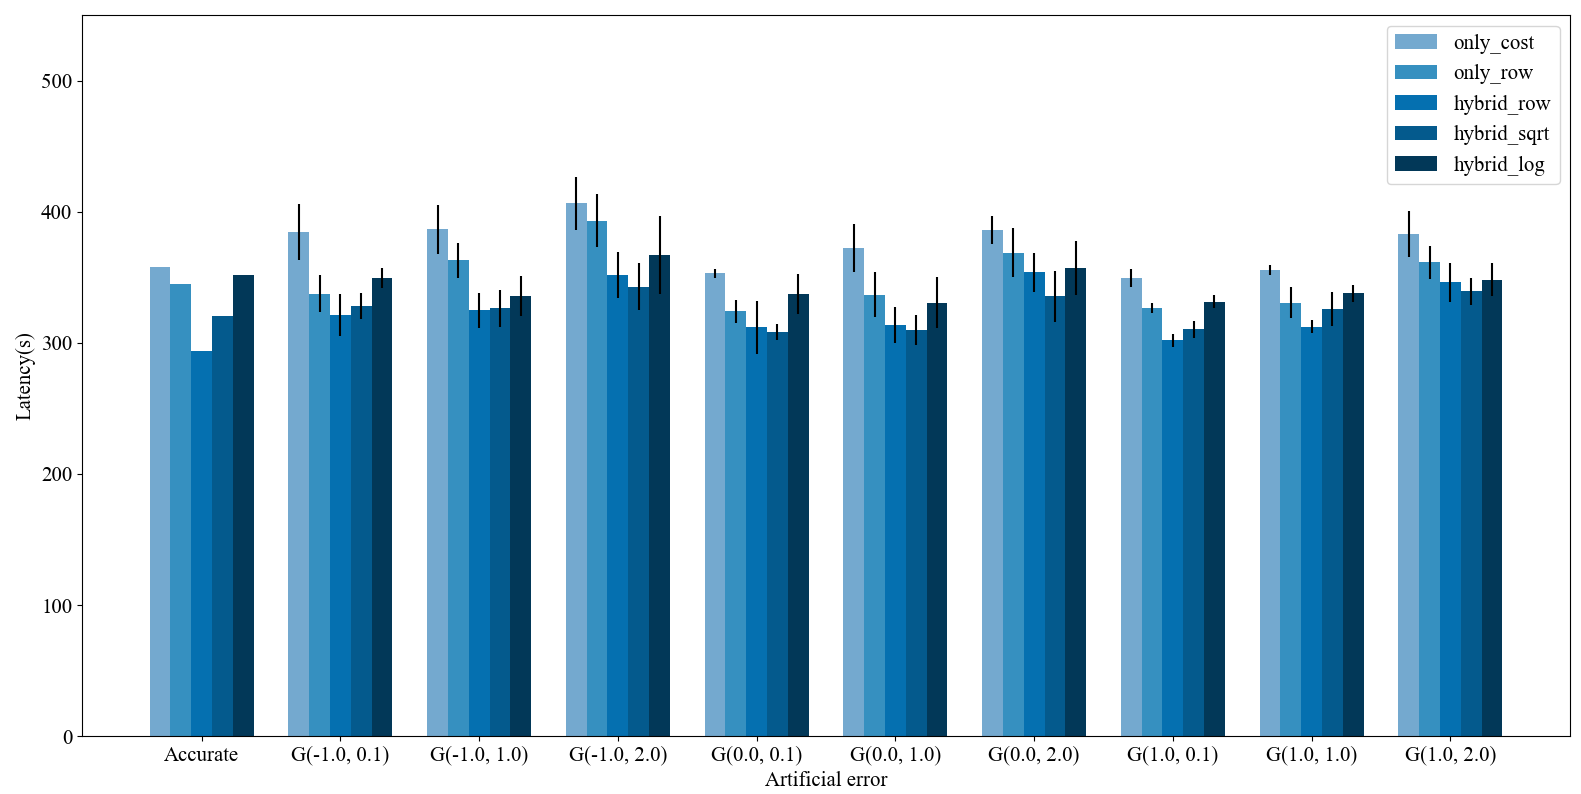
\includegraphics[width=\linewidth]{./pic/Figure9.png}
        \centering
        \caption{Latency of different heuristic-based algorithms under true cardinality and different cardinality estimation error}
        \label{F9}
        \Description{}
    \end{figure*}\par

\subsection{Performance of Query Split} \label{S54}
\textcolor{blue}{
    We further compare \textit{query split} with several baselines. They are 
    \begin{itemize}[leftmargin = 15pt]
        \item Original PostgreSQL.
        \item Optimal optimizer: we have described optimal optimizer above.
        \item Reopt. \cite{Reopt}: A re-optimization technique that only materializes blocked operators and then re-optimizes.
        \item Pop \cite{Pop}: A re-optimization technique materializes both blocked operators and outer sides of nest-loop join.
        \item Query incremental execution (QIE) \cite{QIE}: A re-optimization technique materializes the operator that has the highest cardinality estimation error.
        \item Perron19': A re-optimization technique, which is a brief implementation of the simulation conducted by Perron et al \cite{MichaelStonebraker}. Materializes the nodes that join two relations at a time and then re-optimizes.
        \item USE \cite{USE}: A cardinality estimation technique. Executing the non-expanding operators (i.e., filters and Pk-Fk joins) first and selecting join order by the upper bound of the join instead of cardinality.
        \item Pessimistic CE \cite{PessimisticCE}: A cardinality estimation technique. A worst-optimal cardinality estimator leverages randomized hashing and data sketching to estimate the upper bounds of join size. And using that upper bound to replace the role of cardinality in query optimization. 
    \end{itemize}
}\par
    According to above conclusion, we choose \textit{RelationshipCenter} with $hybrid\_row(q)$ to represent \textit{query split} in the rest of paper, which has the least total end-to-end latency among all implementations.\par
\textcolor{blue}{
    As some source codes of these baselines are not implemented in PostgreSQL, we implement them in PostgreSQL by ourselves according to their algorithms. The parameter configuration is the same as the experiment setup in their paper.
}\par
\textcolor{blue}{
    Figure \ref{F10} and \ref{F11} show the total latency of \textit{query split} and above baselines in two kinds of JOB. One is only the indexes on primary key attributes are available (JOB with Pk index) and another is indexed on both primary key and foreign key (JOB with Pk + Fk index). We set a timeout of total latency as 1000 seconds.
}
    \begin{figure}[htb]
        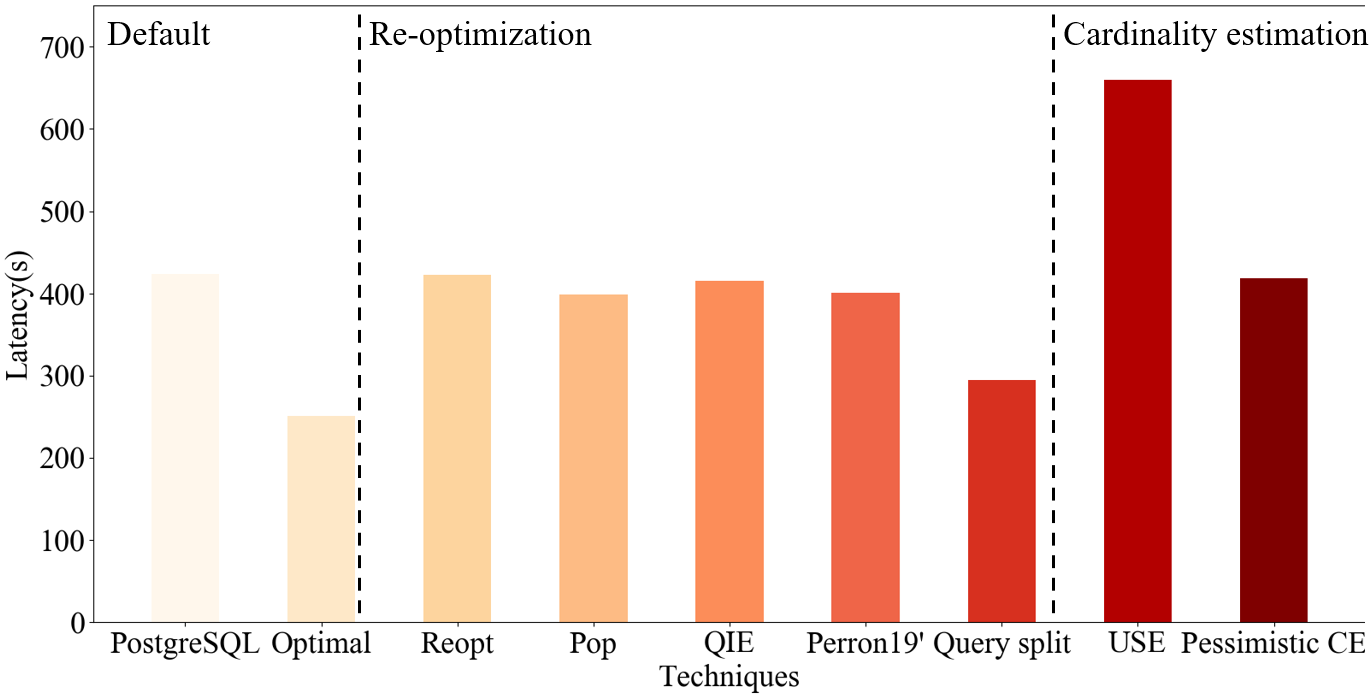
\includegraphics[width=\linewidth]{./pic/Figure10.png}
        \centering
        \caption{Total latency comparison in JOB with Pk + Fk index}
        \label{F10}
        \Description{}
    \end{figure}
    \begin{figure}[htb]
        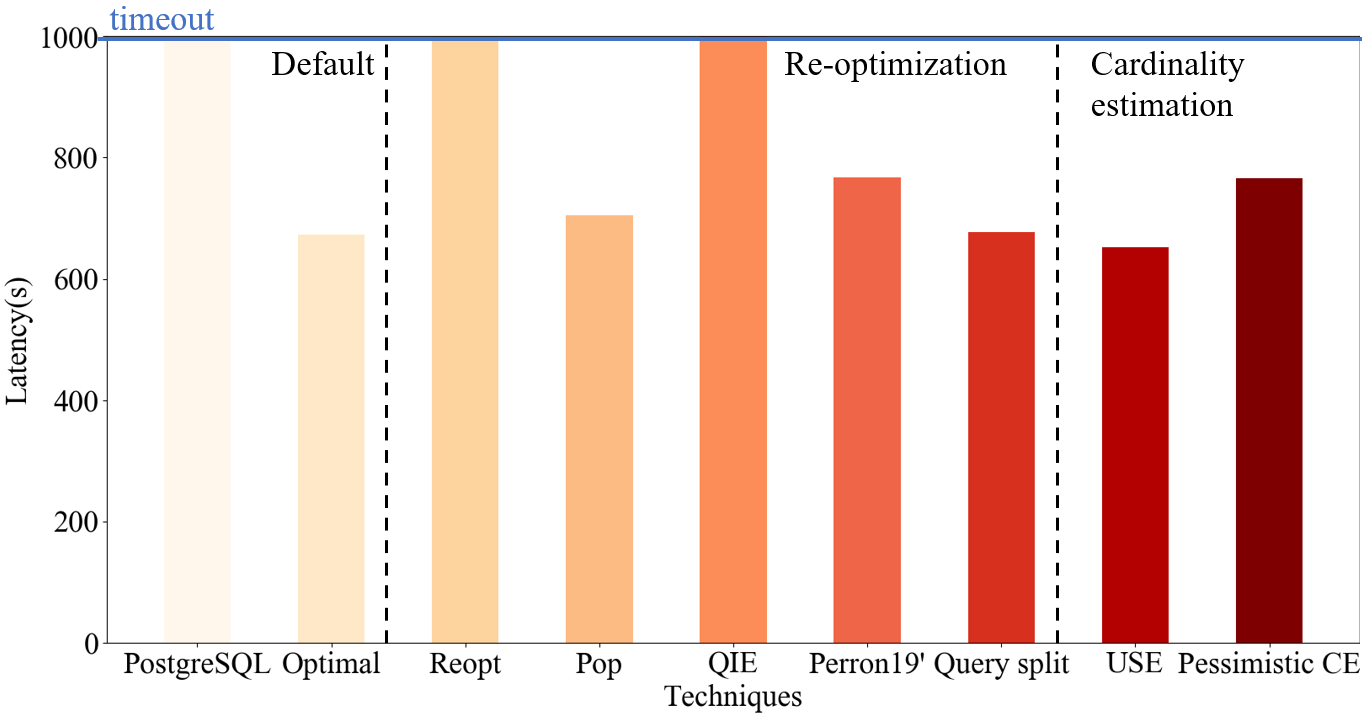
\includegraphics[width=\linewidth]{./pic/Figure11.png}
        \centering
        \caption{Total latency comparison in JOB with Pk index}
        \label{F11}
        \Description{}
    \end{figure}\par
\textcolor{blue}{
    We can draw two conclusions from the above figures. First, \textit{query split} outperforms other query processing techniques. In both Pk-indexed JOB and Pk + Fk indexed JOB, \textit{query split} has a significant speedup for total latency compared to PostgreSQL, other re-optimizations, and new cardinality estimation techniques, which verifies the effectiveness of \textit{query split}. And \textit{query split} is very close to the optimal result. Although there is still a gap between \textit{query split} and \textit{optimal plan} in Pk + Fk indexed JOB, the gap is mainly caused by a few queries, whereas the latency of other queries in \textit{query split} is close to \textit{optimal plan}. And another reason is that the more indexes are available, the harder the job of the query optimizer becomes \cite{JOB}. The result suggests that by proper splitting algorithm and execution order decision, the plans we execute each iteration are more similar to sub-trees of the optimal plan.
}\par
\textcolor{blue}{
    Second, no index on foreign key attributes increases the cost of a bad plan, and therefore the effect of misleading global plans is revealed. The techniques that have the best performance in JOB with Pk index are USE and query split, which both discard the global plan totally. And other re-optimization techniques do not perform well because they are more or less influenced by the terrible part of the global plan.
}\par
    Another implication is that the accuracy of cost model would affect the system performance. We observe that in JOB (Pk index), the latency of \textit{optimal plan} is longer than USE. The reason for this counter-intuitive phenomenon is that the estimation error of cost model, which leads the optimizer to select a sub-optimal physical operator. As the number of configuration parameters that can be tuned in PostgreSQL is limited, it is impossible to tune a perfect cost model. The issue of cost model accuracy is beyond the scope of this paper, and we merely point it out as a potential direction for future research.

\subsection{Materialization Overhead} \label{S55}
\textcolor{blue}{
    All re-optimizations need to materialize the intermediate results as temporary tables. Hence, materialization overhead is an important metric of re-optimization.
}\par
\textcolor{blue}{
    We test the average memory used for materializing the intermediate results of all re-optimization techniques as materialization overhead, and the results are shown in Table \ref{T4}. And we use JOB with Pk + Fk index for the experiment.
}
    \begin{table*}[htb]
        \caption{Materialization overhead of re-optimization techniques}
        \label{T4}
        \begin{tabular}{c|c|c|c}
            \toprule
            Re-optimizations       &  Average overhead & Average re-optimize times & Memory consumption per materialization \\
            \midrule
            \textit{Query split}   &     15.401 MB     &            2.66           &  5.79 MB \\
            Perron19'              &     72.445 MB     &            6.59           & 10.99 MB \\
            Reopt                  &      9.096 MB     &            0.21           & 43.31 MB \\
            Pop                    &     32.396 MB     &            4.62           &  7.01 MB \\
            QIE                    &     45.380 MB     &            3.11           & 14.59 MB \\
            \bottomrule
        \end{tabular}
    \end{table*}\par
\textcolor{blue}{
    From Table \ref{T4}, we can see that \textit{query split} and reopt have low average materialization overhead. However, the overhead of reopt is low because re-optimization is triggered rarely in these two re-optimization techniques. Hence, by calculating the memory consumption per materialization, we find that \textit{query split} has the most efficient memory usage. This is because \textit{query split} controls the result size of sub-query by a specially-designed splitting algorithm, while other re-optimization techniques fail to control the intermediate result sizes.
}

\subsection{Collecting different Run-time Statistics} \label{S56}
\textcolor{blue}{
    The run-time statistics we discuss in the paper include the true cardinality and fine-grained statistics like the most common values, histogram, or the number of distinct values. An interesting question is whether those fine-grained statistics are indispensable for refining execution plans, and we discuss this question in this subsection.
}\par
\textcolor{blue}{
    We test all the re-optimization techniques with and without collecting fine-grained statistics after each materialization. Without collecting fine-grained statistics, the optimizer only knows the size of the intermediate result. As we described before, fined-grained statistics are collected by calling the functions used by PostgreSQL ``analyze" command. The latency of JOB with or without fine-grained statistics is shown in Figure \ref{F12}, and we use JOB with Pk + Fk index for the experiment.
}
    \begin{figure}[htb]
        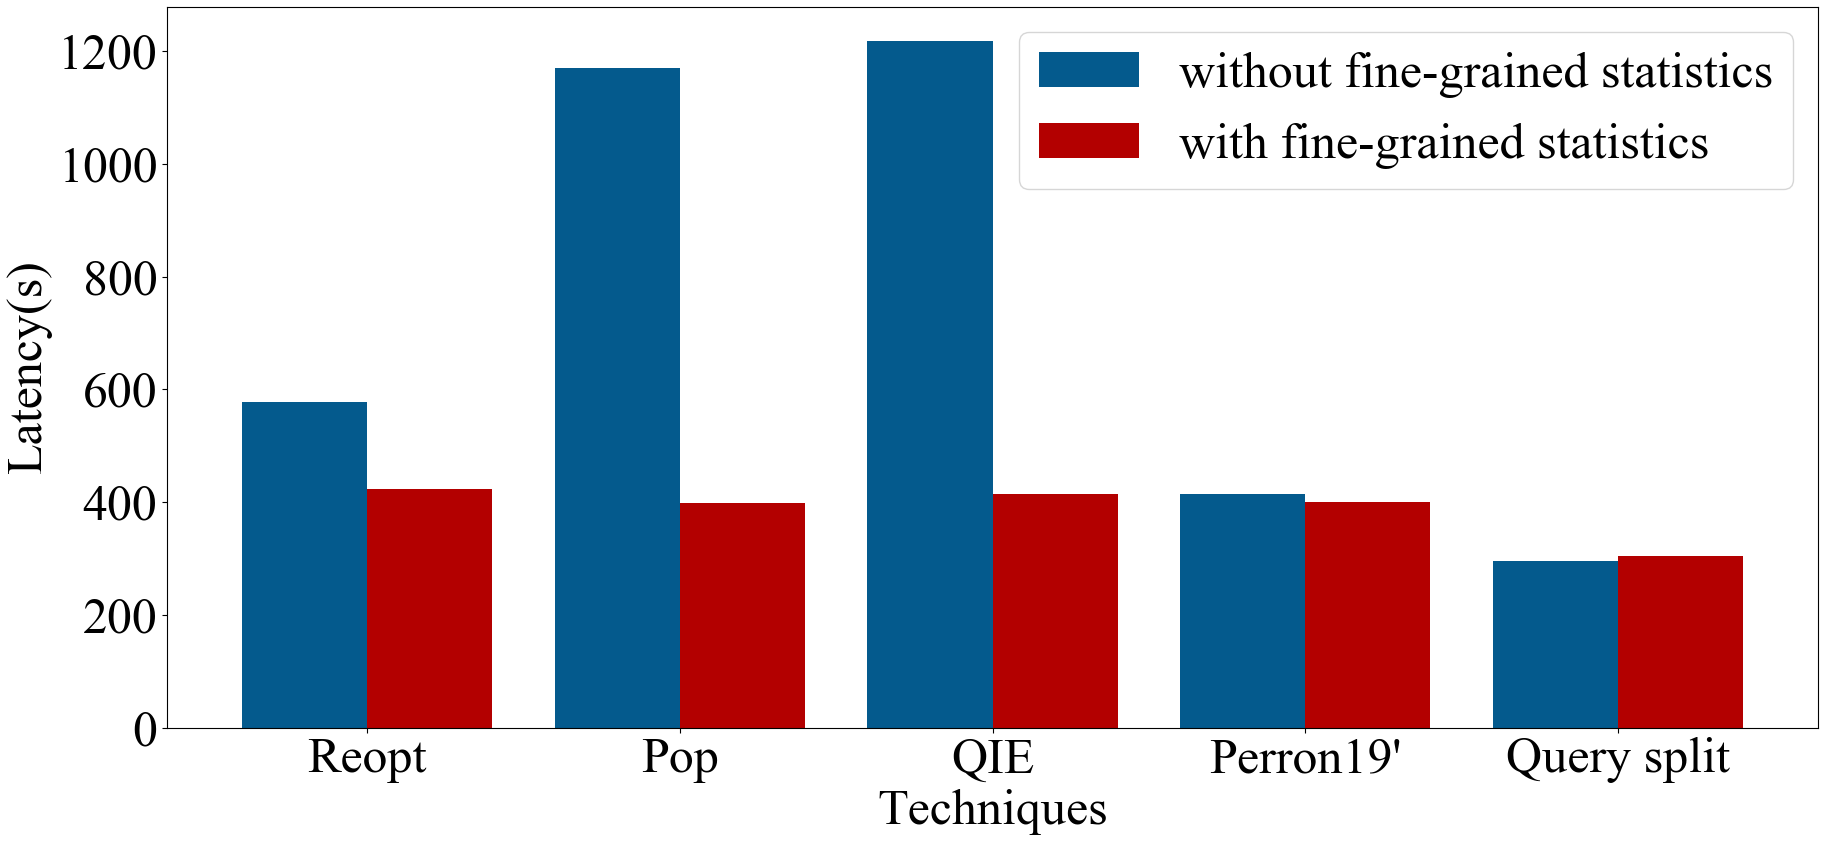
\includegraphics[width=\linewidth]{./pic/Figure12.png}
        \centering
        \caption{Total latency with and without fine-grained statistics}
        \label{F12}
        \Description{}
    \end{figure}\par
\textcolor{blue}{
    From Figure \ref{F12}, we can see that \textit{query split} and Perron19' perform well even without fine-grained statistics during run-time. However, most re-optimization techniques depend heavily on fine-grained statistics to help refine the remaining query.
}

\section{Deal with non-SPJ Query} \label{S6}
    In this section, we discuss how to extend \textit{query split} to handle queries that contain other operations (e.g. outer join, semi join, or aggregation functions). We first give an overview of the extended \textit{query split} in Section 6.1, then introduce how to get the result of non-SPJ operations in Section 6.2. Although we have not implemented the support for these kinds of queries, the basic underlying ideas are quite straightforward. 
\subsection{Overview} \label{S61}
    To deal with non-SPJ queries, the basic idea is to split them into non-SPJ operations that connect several SPJ sub-queries and apply \textit{query split} on each sub-query.\par
    The workflow of the extended algorithm is shown in Figure \ref{F13}. If the query \textbf{Q} is a SPJ query, we simply run standard \textit{query split} on it. Otherwise, we process \textbf{Q} as follows:
    \begin{enumerate}[leftmargin = 15pt]
        \item We parse the query, and select a non-SPJ operator (denote as \textbf{op}) with maximal depth, such that all its inputs are SPJ queries.
        \item We obtain the result of \textbf{op} by the methods that we will describe in Section 6.2. 
        \item We generate a new query \textbf{Q'} from \textbf{Q} by regarding the result of \textbf{op} as a base relation.
        \item Repeat (1)-(3) on \textbf{Q'} until it becomes a SPJ query.
    \end{enumerate}
    \begin{figure}[htb]
        \centering
        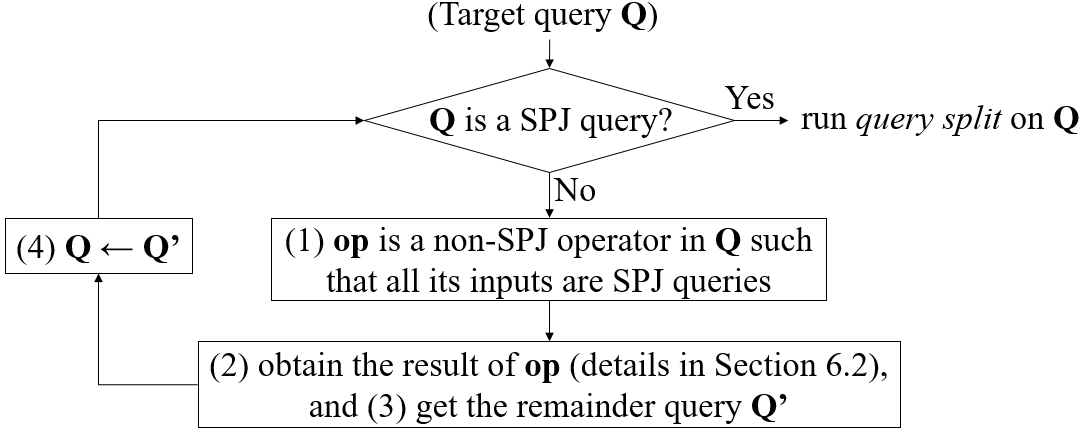
\includegraphics[width=\linewidth]{./pic/Figure13.png}
        \caption{The workflow of extended \textit{query split}}
        \label{F13}
        \Description{}
    \end{figure}

\subsection{Execute non-SPJ Operators} \label{S62}
    To obtain the result of a non-SPJ operator, we first construct the input sub-queries and execute them via \textit{query split}. Then, we deliver the sub-query results to the non-SPJ operator and execute it.\par
    As shown in Figure \ref{F14}, to deliver the sub-query results to the non-SPJ operator, we can choose either pipelining one tuple at a time or materializing the entire result. Note that this is different from standard \textit{query split}, since it is not necessary to gather run-time statistics. Although the run-time statistics can be used for choosing a better physical operator, the benefit of doing this is often very limited.
    \begin{figure}[htb]
        \centering
        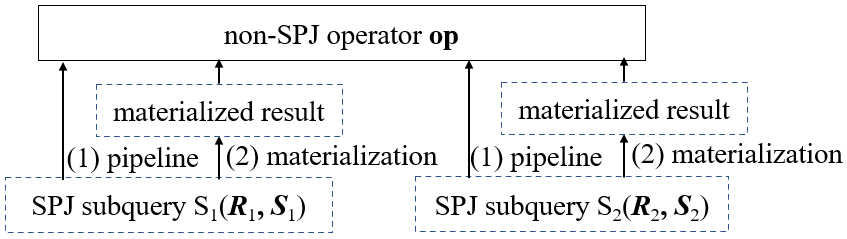
\includegraphics[width=\linewidth]{./pic/Figure14.png}
        \caption{Sub-queries of a non-SPJ operator}
        \label{F14}
        \Description{}
    \end{figure}

\section{Case Study} \label{S7}
    In this section, we choose two example queries (in Section \ref{S71} and \ref{S72}) from JOB as case study to obtain some insights into \textit{query split}. We demonstrate the detailed execution plan of \textit{query split} on these queries by Figure \ref{F15} and \ref{F16}, and explain what makes \textit{query split} faster than PostgreSQL, then discuss our findings from case studies in Section \ref{S73} and Section \ref{S74}.\par
Before analyzing the examples, we introduce the marks that will appear in the figures. In Figure \ref{F15} and \ref{F16}, the percentage next to the execution node represents the ratio of the time spent by the physical operator to the \textbf{total execution time} of \textit{query split}. The colored line represents the boundary of subqueries. The number above the relational algebra represents the estimated and actual size of intermediate results. As the estimation results at the subquery boundaries are precise, we just show the actual value.

\subsection{The First Case} \label{S71}
    \begin{figure}[htb]
        \subfigure[The join graph of example query 1]
        {
            \begin{minipage}[t]{0.9\linewidth}
                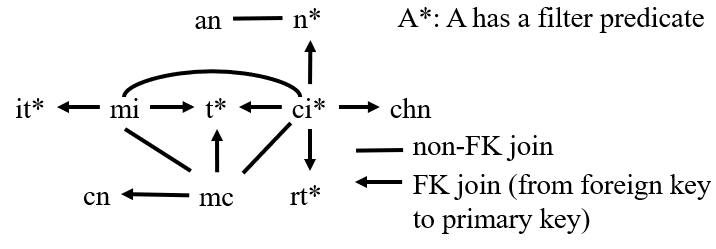
\includegraphics[width=\linewidth]{./pic/Figure15a.png}
            \end{minipage}
        }
        \subfigure[Execution plan of PostgreSQL]
        {
            \begin{minipage}[t]{0.47\linewidth}
                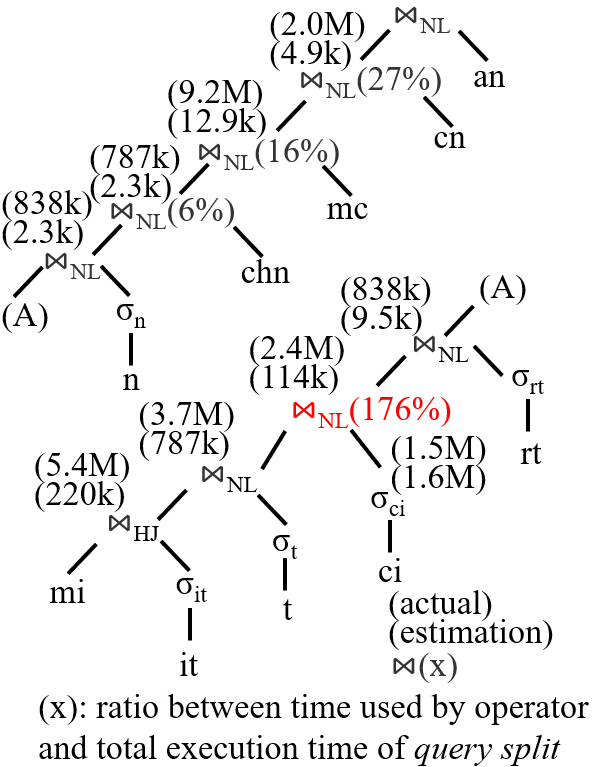
\includegraphics[width=\linewidth]{./pic/Figure15b.png}
            \end{minipage}
        }
        \subfigure[Execution plan of \textit{query split}]
        {
            \begin{minipage}[t]{0.47\linewidth}
                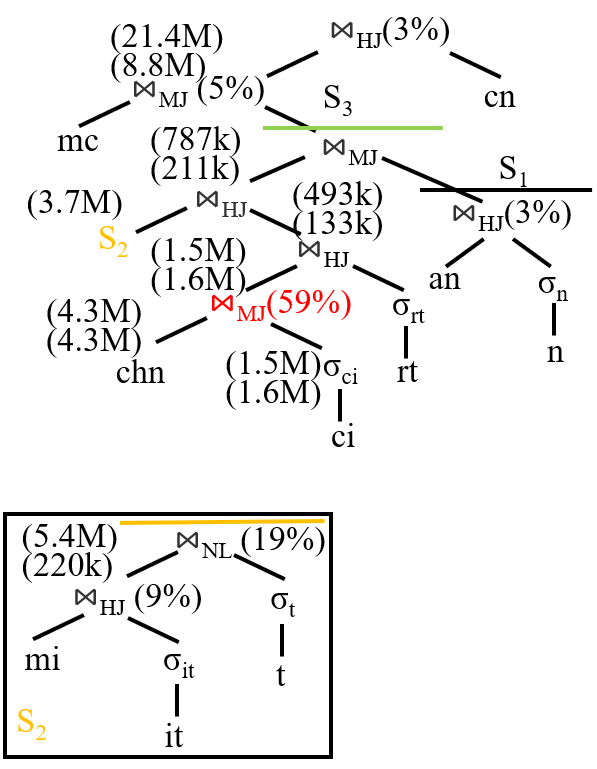
\includegraphics[width=\linewidth]{./pic/Figure15c.png}
            \end{minipage}
        }
        \centering
        \caption{The detail of query execution for example 1}
        \label{F15}
        \Description{}
    \end{figure}\par
    As shown in Figure \ref{F15}, there is a big gap between the cardinality estimation errors in PostgreSQL and query split. We use q-error \cite{paper53}, the factor by which the estimation differs from the true cardinality, to measure the quality of cardinality estimation. The average q-error in PostgreSQL is 246, while in \textit{query split} it is only 5.\par
    Another major difference in the execution plan between PostgreSQL and \textit{query split} is about how to deal with the join with table \textbf{ci}. In PostgreSQL, the execution plan directly join \textbf{ci} with the current intermediate result by nest loop. However, it's unwise because both left and right subtree are huge. As shown in Figure \ref{F15}(b), this nest loop costs too much time. In contrast, the decision of \textit{query split} is much better. As shown in Figure \ref{F15}(c), execution plan in \textit{query split} first decreases the size of table \textbf{ci} by joining with entity relations \textbf{chn} and \textbf{rt}. Note that although \textbf{chn} is huge as well, merge join can be applied without sorting and use much less time. Then, after the size of \textbf{ci} is reduced, it is joined with $S_2$. This decision effectively improves a time-consuming join in PostgreSQL and speeds up the query execution (from 128s to 48s).

\subsection{The Second Case} \label{S72}
    \begin{figure}[htb]
        \subfigure[The join graph of example query 2]
        {
            \begin{minipage}[t]{0.9\linewidth}
                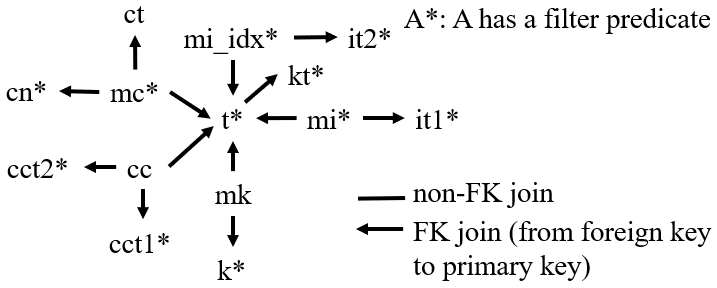
\includegraphics[width=\linewidth]{./pic/Figure16a.png}
            \end{minipage}
        }
        \subfigure[Execution plan of PostgreSQL]
        {
            \begin{minipage}[t]{0.47\linewidth}
                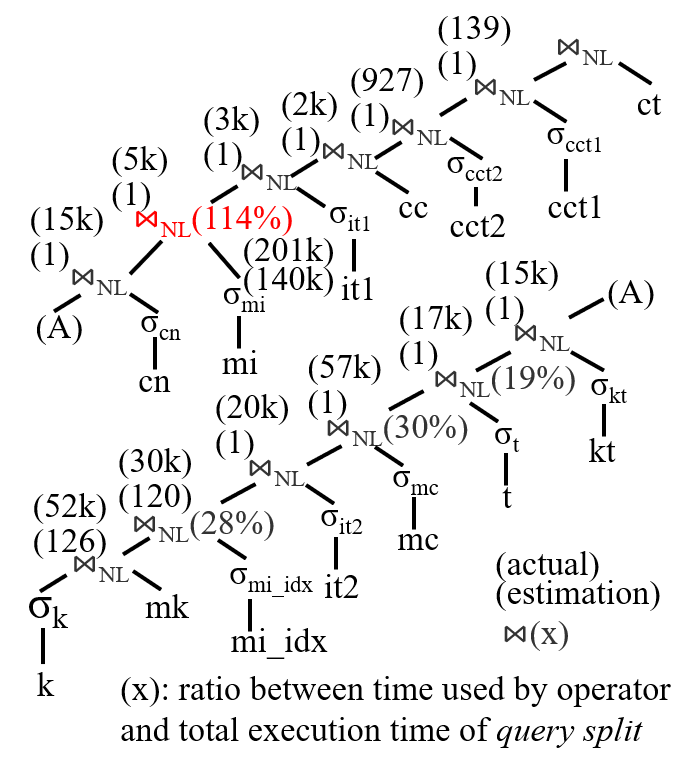
\includegraphics[width=\linewidth]{./pic/Figure16b.png}
            \end{minipage}
        }
        \subfigure[Execution plan of \textit{query split}]
        {
            \begin{minipage}[t]{0.47\linewidth}
                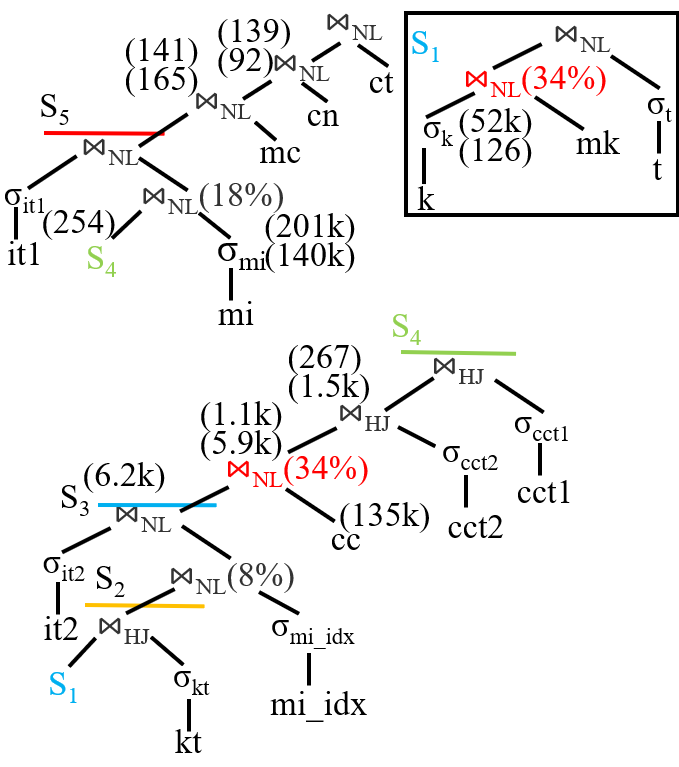
\includegraphics[width=\linewidth]{./pic/Figure16c.png}
            \end{minipage}
        }
        \centering
        \caption{The detail of query execution for example 2}
        \label{F16}
        \Description{}
    \end{figure}\par
    As shown in Figure \ref{F16}, there is also a big gap between the cardinality estimation errors in PostgreSQL and query split. The average q-error in PostgreSQL is 11310, while in \textit{query split} it is 37.\par
    Figure \ref{F16}(b) illustrates that the poor performance of PostgreSQL is due to using too much time to join table \textbf{mi}, where two huge inputs are involved. As shown in Figure \ref{F16}(c), in \textit{query split}, the optimizer postpones the join with \textbf{mi}, and instead decreases the size of inputs first. So when the join with \textbf{mi} happens in \textit{query split}, the size of another input is relatively small, which makes the execution faster.

\subsection{Our Findings} \label{S73}
    Now we can generalize two findings from case studies. First, the plan produced by \textit{query split} is close to \textit{optimal plan}. This is due to two reasons:
    \begin{itemize}[leftmargin = 15pt]
        \item The execution plan in each subquery is near-optimal. By gathering run-time statistics after the execution of each subquery, optimizer can get precise statistics of base relations in subqueries. Meanwhile, the size of each subquery is small. Under such conditions, cardinality estimation of the database optimizer is relatively accurate.
        \item By considering both result size and execution time, we can make a decent decision on subquery execution order. We postpone the execution of long-time join and decrease its size by replacing original inputs with other subqueries' results.
    \end{itemize}\par
    Second, we find that both queries are dominated by a very slow physical operator that consumes a massive piece of time (i.e. merge join and nest loop join), which takes more than half of the total execution time. We study this topic further in Section \ref{S74} to reveal remaining bottlenecks of query execution when the join order is good enough, and thus can help us further improve the query execution performance.

\subsection{A Further Study on Physical Operator} \label{S74}
    The phenomenon that the execution time is dominated by a single physical operator is in fact quite common in JOB. To study this topic further, we classify queries in JOB according to the operator that takes the longest time during execution, as shown in Table \ref{T5}.
    \begin{table}[htb]
        \caption{The physical operators that dominate JOB queries}
        \label{T5}
        \begin{tabular}{c|m{5cm}}
            \toprule
            physical operator & query Ids \\
            \hline
            hash join & 16, 23, 24, 28, 30, 55, 61, 81 \\
            \hline
            merge join & 46, 54 \\
            \hline
            index scan & 1, 2, 3, 4, 5, 6, 7, 8, 9, 10, 11, 12, 13, 15, 17, 19, 20, 21, 22, 29, 31, 32, 33, 34, 35, 36, 37, 38, 39, 40, 42, 45, 46, 47, 48, 49, 53, 56, 57, 62, 63, 64, 65, 66, 67,68, 69, 70, 71, 72, 73, 74, 75, 76, 77, 78, 79, 80, 82, 83, 84, 85, 86, 87, 88, 89, 90, 91 \\
            \hline
            sequential scan & 14, 18, 25, 26, 27, 41, 43, 44, 50, 51, 52, 58, 59, 60 \\
            \bottomrule
        \end{tabular}
    \end{table}\par
    We find that most queries are dominated by an index scan and other queries are dominated by hash join, merge join, or sequential scan.\footnote[4]{Note that our conclusion is derived from JOB, in which the number of queries is limited, and queries are human-write. The above reasons may cause our conclusion to be particular for JOB but not general for other benchmarks.} In the following part, we will discuss each of these operators.

    \subsubsection{Hash Join and Merge Join}
        It is possible further improve \textit{hash join} and \textit{merge join} by using a new and faster physical operator, \textit{directmap join}. In \textit{hash join}, to fetch an inner tuple, we need two random memory accesses: one for probing the hash table, another for accessing the inner tuple. If we reduce the number of memory accesses to once, we can achieve a faster execution speed.\par
        By combining probing and accessing data together, \textit{directmap join} can fetch a matching inner tuple through one memory access. Like \textit{hash join}, \textit{directmap join} consists of two phases: build phase and probing phase. In build phase, we copy the data of inner relation into a two-dimension array called \textit{map}, which can be treated as a combination of hash table and relation data. Due to the join attribute values in JOB being non-negative integer and having limited range, we simply use the original value as hash value ($hash(x)=x$), and each row of \textit{map} is used to store an inner tuple.
        \begin{figure}[htb]
            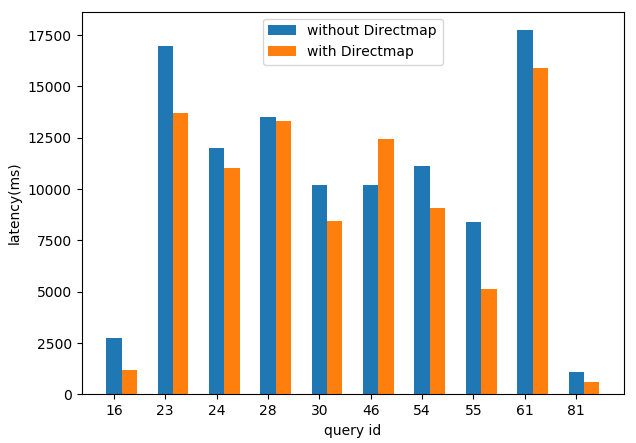
\includegraphics[width=\linewidth]{./pic/Figure17.png}
            \caption{The effect of \textit{directmap} on queries with join operator bottleneck}
            \label{F17}
            \Description{}
        \end{figure}\par
        In probe phase, for each tuple from outer relation with join attribute value $x$, we fetch the corresponding row $\textit{map}[x]$ and return the inner tuple if it is not empty. In this way, when probing and accessing an inner tuple, we only use one random memory access. We will explain the detailed implementation of \textit{directmap join} in Appendix \ref{A3}.\par
        We use \textit{directmap join} in those join operator constraint queries, and compare their execution time with previous results. The end-to-end latencies are shown in Figure \ref{F17}. Query 16, 55 and 81 have more than 50\% improvement in end-to-end latency, and query 23, 30 and 54 have nearly 25\% improvement. The result proves that \textit{directmap join} can greatly improve the total execution time for queries with join operator as bottleneck.
        

    \subsubsection{Index Scan and Sequential Scan}
        Unlike hash join and merge join, the queries dominated by \textit{index scan} and \textit{sequential scan} are hard to improve due to three reasons:
        \begin{enumerate}[leftmargin = 15pt]
            \renewcommand{\labelenumi}{\theenumi.}
            \item The use of scan operators is inevitable. 
            \item As far as we know, apart from \textit{index scan} and \textit{sequential scan}, there are no other comparable scan operators. In other words, if the optimizer has chosen the better scan operator between \textit{index scan} and \textit{sequential scan}, then there is little room for further improvement. 
            \item According to the cost model in PostgreSQL \cite{manual2}, we substitute the true cardinality into the cost model and find the scan operator decision made by the optimizer is indeed correct in \textit{query split}.
        \end{enumerate}\par
        From above three points, we conclude that there is no room to further improve \textit{index scan} and \textit{sequential scan} in \textit{query split}. Hence, under the dynamic query optimization framework, for most queries dominated by a scan operator, \textit{query split} is already a nearly optimal solution. Although there might exist some other strategies to further improve scan operators, such strategy are beyond the scope of our paper.
    
\section{Related Work} \label{S8}
    Our work is relevant to three research directions: (a) the literatures that studies the intrinsic difficulty of accurate cardinality estimation; (b) adaptive query processing \cite{paper57}; (c) researches that aim to improve accuracy of cardinality estimation. We state existing works in these directions respectively in Section \ref{S81}, \ref{S82}, and \ref{S83}.
\subsection{Difficulty of Cardinality Estimation} \label{S81}
    On theoretical front, Yannis and Stavros \cite{paper31} proved that cardinality estimation errors would grow exponentially with join size. They study the natural join and assume there is an error on the estimated distribution of join attributes in each relation.\par
    Leis et al. \cite{JOB} pay attention to practice and use experiments to show that cardinality estimators in commercial database produce large errors in real workload. They introduced a new benchmark called ``Join Order Benchmark", which is simple but challenging. Their experiments suggest that although cardinality estimator is accurate for one relation queries, no existing techniques can accurately estimate cardinality with high correlated join predicates.\par
    Their research shows the necessity for new query optimization frameworks and the intrinsic difficulty of accurate cardinality estimation, which inspires our research on dynamic query optimization.

\subsection{Adaptive Query Processing} \label{S82}
    According to reference \cite{paper47}, there are three families in adaptive query processing: plan-based system (re-optimization), routing-based system and continuous-query-based system.  
    
    \subsubsection{Re-optimization} The most relevant work in the literature is re-optimization. Re-optimization monitors the execution of the current plan and re-optimizes whenever the actual condition differs significantly from the estimations made by the optimizer.\par
    \textit{Reopt} \cite{Reopt} and \textit{Pop} \cite{Pop} are the two most representative works on re-optimization. \textit{Reopt} adds statistic collection operators to the execution plan and collects statistics after a segment has been executed. When finding that the collected statistic deviates too much from estimation, the database triggers re-optimization and re-optimizes the unexecuted part by the collected statistic.\par
    The idea of \textit{Pop} is the same as \textit{Reopt}, but \textit{Pop} can trigger re-optimization in more join nodes, like the outer side of nest-loop join, while \textit{Reopt} can only trigger re-optimization at the blocked operator.\par
    Conquest \cite{paper39} extends the re-optimization to a parallel execution environment. Query incremental execution \cite{QIE} estimates the error of cardinality estimation at each operator and materializes the operator that has the largest error currently. To decrease the time of collecting the intermediate statistics, sampling re-optimization \cite{SampleReopt} throws the plan to sampling-based estimator. In recent work, Cuttlefish \cite{paper29} uses reinforcement learning techniques to explore possible physical operators during query execution and exploits the fastest ones. However, Cuttlefish can only modify the physical operator, but is unable to change the join order.\par
    Recently, Perron et al. \cite{MichaelStonebraker} simulates re-optimization in PostgreSQL. They first observe the error by the ``explain" command and materialize the intermediate result that deviates too much from estimation as a temporary table. Then they rewrite the query by replacing the materialized part with the temporary table, and finally they call the optimizer again. Their result shows that re-optimization in PostgreSQL can sharply improve the execution time.\par
\textcolor{blue}{
    Compared to the \textit{query split} framework, the query execution of the above re-optimizations is still based on the global plan. And if the global plan is terrible, re-optimization's sub-plan can also be terrible. Note that the first time of materialization in re-optimization is before the first re-optimization is triggered. Hence, if the sub-plan we choose initially is a sub-optimal plan, we lose the opportunity to correct this wrong decision.
    }
    
    \subsubsection{Routing-based system} Routing-based systems eliminate the traditional optimizer and query plans. They process queries by routing tuples through a pool of operators. The idea of the routing-based system can be traced back to INGRES \cite{paper46}. In INGRES, each tuple could be executed in a different order. The routing-based system eliminates the concept of execution plan by routing tuples one by one. Eddies \cite{paper30} adds a new operator called ripple join, and Eddies can change the join order in ripple join.\par
    Both re-optimization and routing-based system break the unidirectional pipeline between optimizer and executor. However, compared to re-optimziation, routing-based systems totally abandon optimizer, making routing algorithms highly dependent on greedy algorithm and therefore unsuitable for complex queries \cite{paper47}.
    
    \subsubsection{Continuous-query-based System} Continuous-Query-based, or CQ-based, systems are used for queries that will run many times or a very long time, which is prevalent in the data stream systems.\par
    Although CQ-based systems also support variable execution plan during execution, however, there is a huge gap between CQ-base systems and our work. CQ-base systems pay attention to the run-time change of stream characteristics and system conditions, rather than cardinality estimation error for a given query.
    
    \subsubsection{Others} Dynamic query plan \cite{paper25, paper42, paper43} and parametric query optimization \cite{paper44} are proposed to change the query plan without calling the optimizer again. They give a set of possible optimal plans to the executor instead of giving one single optimal plan and during execution, the plans can switch to each other.\par
    Similar to other adaptive query processing techniques, these works also pay attention to a flexible execution plan. But compared to our work, query optimization and execution in dynamic query plan and parametric query optimization is not interleaved, which leads to a great overhead to maintain multiple execution plans.

\subsection{Cardinality Estimation} \label{S83}
    Cardinality estimation techniques \cite{paper33} are also relevant. The researches in cardinality estimation techniques aim to improve cardinality estimation. There are two main research areas: data-driven cardinality estimator \cite{paper1, paper5, paper8, paper9, paper17, paper19, paper21, paper22, paper23, paper36}, query-driven cardinality estimator \cite{paper12, paper14, paper15, paper16, paper18, paper34, paper37}. The data-driven cardinality estimator approximates the data distribution of a table by mapping each tuple to its probability of occurrence in the table. The query-driven cardinality estimator uses some models to learn the mapping between queries and cardinalities.\par
    We emphasize that there is no conflict between dynamic query optimization and advanced cardinality estimation techniques. On the contrary, \textit{query split} benefits from the improvement of cardinality estimation on small join. Making an optimal plan in each sub-query can significantly enhance overall performance.\par
\textcolor{blue}{
    One related work is USE \cite{USE} because we both execute the query by sub-query form and use the same idea that uses Pk-Fk join in constraining the sub-queries size. USE pushed the non-expand operators (i.e., filter and Pk-Fk join) to the sub-query, similar to our \textit{RelationshipCenter}. It then used sketch-based cardinality estimation to decide the join order between sub-queries. However, USE is not an adaptive query processing method, and sketch-based cardinality estimation needs pre-processing of the dataset.
}

\section{Conclusion} \label{S9}
    \textcolor{blue}{
    Re-optimization can help the database optimizer avoid the intrinsic difficulty of cardinality estimation. But current re-optimization still needs the global plan to start the initial query execution, which can cause a sub-optimal execution procedure before re-optimization is triggered. In this paper, we propose \textit{query split}, a re-optimization framework with the new sub-query perspective. Discarding the global plan and proactively interleaving query optimization and execution, \textit{query split} reaches near-optimal latency in Join Order Benchmark. Our results suggest that the sub-query perspective can avoid misleading global plans and improve query execution speed. Furthermore, the case study shows that the latency of most queries is dominated by one physical operator. The result implies that the execution time on the query can be hugely improved by improving the bottleneck operator itself. There is little room for further improvement under the re-optimization framework.
}
    
\bibliographystyle{ACM-Reference-Format}
\bibliography{ref}

\appendix
\section{Equivalence Rule}
    This appendix shows the concrete formulas that can be used to obtain the normal form of SPJ query. Because all select-projection-join queries are relational algebra expressions that consist of only select, projection and join, we can transform them to a normal form by equivalence rule:\par
    \begin{itemize}[leftmargin = 15pt]
        \item For each join expression, we can rewrite it as select after Cartesian product:
        $$ r_1 \bowtie_{\theta} r_2=\sigma_{\theta}(r_1 \times r_2) $$
        \item We can change the order between projection and Cartesian product:
        $$ \Pi_{A}(r_1) \times \Pi_{B}(r_2)=\Pi_{A \cup B}(r_1 \times r_2) $$
        where $A$ and $B$ are the set of attributes.
        \item We can change the order between select and Cartesian product:
        $$ \sigma_{A}(r_1) \times \sigma_{B}(r_2)=\sigma_{A \cup B}(r_1 \times r_2) $$
        where $A$ and $B$ are the set of predicates.
        \item When select is executed after projection, we can change their orders:
        $$ \sigma_{B}(\Pi_{A}(r_1))=\Pi_{A}(\sigma_{B}(r_1)) $$
        where $A$ is the set of attributes and $B$ is the set of predicates.
    \end{itemize}\par
    By above four transformations, we move all select operations after all Cartesian products, and move projections after all select operations, which is the normal form of SPJ query. \label{A1}
\section{Proof of Theorem 1}
    This appendix shows the proof of Theorem 1.
    \begin{Theorem}
        Let q(\textbf{\textit{R}}, \textbf{\textit{S}}, \textbf{\textit{P}}) be an SP$J$ query, \textbf{\textit{Q}} be a set of subqueries of q. If \textbf{\textit{Q}}$\rightharpoonup_c$q, then the output of the replacement reconstruction algorithm is equal to the result of q.
    \end{Theorem}
    \begin{Proof}
        \ \newline 
        \indent To begin with, let us introduce several notations:
        \begin{enumerate}[leftmargin = 15pt]
            \item For a set of subqueries $\textbf{\textit{Q}}=\{q_1(\textbf{\textit{R}}_1,\textbf{\textit{S}}_1),...,q_n(\textbf{\textit{R}}_n,\textbf{\textit{S}}_n)\}$, we denote $R(\textbf{\textit{Q}})=\cup_{i=1}^n \textbf{\textit{R}}_i$, $S(\textbf{\textit{Q}})=\cup_{i=1}^n \textbf{\textit{S}}_i$.
            \item For a set of relations $\textbf{\textit{R}}=\{r_1,...,r_n\}$, we denote $\mathsf{X}_{r \in \textbf{\textit{R}}}=r_1 \times ... \times r_n$.
            \item For a SP$J$ query $q(\textbf{\textit{R}},\textbf{\textit{S}},\textbf{\textit{P}})$ and a set of subqueries $\textbf{\textit{Q}}$ of $q$, we denote the result of $q$ as $E(q)=\Pi_{\textbf{\textit{P}}}(\sigma_{\textbf{\textit{S}}}(\mathsf{X}_{r \in \textbf{\textit{R}}}))$, and the output of the replacement reconstruction algorithm as $E(\textbf{\textit{Q}}, \textbf{\textit{P}})$.
        \end{enumerate}\par
        \indent Notice that in both $E(q)$ and $E(\textbf{\textit{Q}}, \textbf{\textit{P}})$, the projection is performed at last over the same projection attribute set $\textbf{\textit{P}}$. Thus if the results before projection are same, the final results are same as well. Therefore, we can simplify notations of (3): For a SP$J$ query $q(\textbf{\textit{R}},\textbf{\textit{S}})$ and the set of subqueries $\textbf{\textit{Q}}$ of $q$, we denote the result of $q$ as $E(q)=\sigma_{\textbf{\textit{S}}}(\mathsf{X}_{r \in \textbf{\textit{R}}})$, and the output of the replacement reconstruction algorithm as $E(\textbf{\textit{Q}})$.
        \indent Under these notations, we can rewrite the theorem as: Given a SP$J$ query $q(\textbf{\textit{R}},\textbf{\textit{S}})$, and a set of subqueries $\textbf{\textit{Q}}$ of $q$, such that $\textbf{\textit{Q}} \rightharpoonup_c q$. Then we have $E(q)=E(\textbf{\textit{Q}})$.\newline
        \indent Without loss of generality, we assume that the names of all attributes in $\textbf{\textit{R}}$ are unique. Under such assumption, we do not need to consider the rename operation when modifying subqueries, and for simplicity we assume that the rename step is skipped.\newline
        \indent Now, we start to prove the rewritten theorem by induction on $|\textbf{\textit{Q}}|$.\newline
        \indent First, We prove the statement holds when $|\textbf{\textit{Q}}|=1$, in which case $\textbf{\textit{Q}}=\{q_1(\textbf{\textit{R}}_1,\textbf{\textit{S}}_1)\}$. Apparently the only way that $\textbf{\textit{Q}} \rightharpoonup_c q$ is $q_1=q$. So the statement clearly holds for $|\textbf{\textit{Q}}|=1$.\newline
        \indent Now, assume that the statement holds when $|\textbf{\textit{Q}}|=n-1$. We consider the case of $|\textbf{\textit{Q}}|=n$, $\textbf{\textit{Q}}=\{q_1(\textbf{\textit{R}}_1,\textbf{\textit{S}}_1),...,q_n(\textbf{\textit{R}}_n,\textbf{\textit{S}}_n)\}$.\newline
        \indent Without loss of generality, we denote the first executed subquery as $q_1(\textbf{\textit{R}}_1,\textbf{\textit{S}}_1)$ and discuss two cases: (1) $\forall i > 1, \textbf{\textit{R}}_1 \cap \textbf{\textit{R}}_i=\emptyset$ and (2) $\exists i > 1, s.t. \textbf{\textit{R}}_1 \cap \textbf{\textit{R}}_i \neq \emptyset$.\newline
        \textbf{Case 1}: We first execute $q_1$ and materialize its result as relation $m_1=E(q_1)$. Then, because $\forall i > 1, \textbf{\textit{R}}_1 \cap \textbf{\textit{R}}_i=\emptyset$, according to the algorithm, we have to add $m_1$ to the subquery result set $\textbf{\textit{L}}$ in \textbf{Loop(modify)} phase. After that, we remove $q_1$ from $\textbf{\textit{Q}}$ and have a new subquery set $\textbf{\textit{Q}}'=\{q_2(\textbf{\textit{R}}_2,\textbf{\textit{S}}_2),...,q_n(\textbf{\textit{R}}_n,\textbf{\textit{S}}_n)\}$ for the next iteration.\newline
        \indent We construct a SP$J$ query $q'(\textbf{\textit{R}}',\textbf{\textit{S}}')$, where $\textbf{\textit{R}}'= \cup_{i=2}^{n} \textbf{\textit{R}}_i$ and $\textbf{\textit{S}}'=\cup_{i=2}^{n} \textbf{\textit{S}}_i$. Apparently, $\textbf{\textit{Q}}' \rightharpoonup_c q'$ and as $|\textbf{\textit{Q}}'|=n-1$, by induction hypothesis, $E(q')=E(\textbf{\textit{Q}}')$.\newline
        \indent  According to \textbf{Merge} phase, final result is the Cartesian product on the elements in $\textbf{\textit{L}}$, so we have:
        $$E(\textbf{\textit{Q}})=\mathsf{X}_{r \in \textbf{\textit{L}}}=m_1 \times \mathsf{X}_{r \in (\textbf{\textit{L}} \setminus \{m_1\})}=E(q_1) \times E(\textbf{\textit{Q}}')=E(q_1) \times E(q')$$
        $$=\sigma_{\textbf{\textit{S}}_1}(\mathsf{X}_{r \in \textbf{\textit{R}}_1}) \times \sigma_{\textbf{\textit{S}}'}(\mathsf{X}_{r \in \textbf{\textit{R}}'})=\sigma_{\textbf{\textit{S}}_1 \cup \textbf{\textit{S}}'}(\mathsf{X}_{r \in \textbf{\textit{R}}})=\sigma_{\textbf{\textit{S}}}(\mathsf{X}_{r \in \textbf{\textit{R}}})=E(q)$$
        \textbf{Case 2}: We denote the set of subqueries that need to be modified after executing $q_1$ as $\textbf{\textit{W}}=\{q_k(\textbf{\textit{R}}_k,\textbf{\textit{S}}_k) \in \textbf{\textit{Q}}:k > 1,\textbf{\textit{R}}_1 \cap \textbf{\textit{R}}_k \neq \emptyset\}$.\newline
        \indent After we execute $q_1$ and materialize its result as relation $m_1$, we modify each $q_i \in \textbf{\textit{W}}$ and keep $\textbf{\textit{L}}=\emptyset$ in \textbf{Loop(modify)} phase. We denote these new-formed subqueries as $q'_i(\textbf{\textit{R}}'_i, \textbf{\textit{S}}'_i)$ and $\textbf{\textit{R}}'_i=\textbf{\textit{R}}_i \setminus \textbf{\textit{R}}_1 \cup \{m_1\}$, $\textbf{\textit{S}}'_i=\textbf{\textit{S}}_i$. These new-formed subqueries form a new set $\textbf{\textit{W}}'$.\newline
        \indent Now, $\textbf{\textit{Q}}$ becomes a new subquery set $\textbf{\textit{Q}}'=\textbf{\textit{Q}} \cup \textbf{\textit{W}}' \setminus \{q_1\} \setminus \textbf{\textit{W}}$. Because $\textbf{\textit{L}} = \emptyset$ at this point, when reconstruction finishes, we have $E(\textbf{\textit{Q}})=E(\textbf{\textit{Q}}')$.\newline
        \indent We construct a new query $q'(\textbf{\textit{R}}',\textbf{\textit{S}}')$, where $\textbf{\textit{R}}'=\textbf{\textit{R}} \setminus \textbf{\textit{R}}_1 \cup \{m_1\}$ and $\textbf{\textit{S}}'=\cup_{i=2}^{n} \textbf{\textit{S}}_i$. We will prove that $E(q')=E(\textbf{\textit{Q}}')$ and $E(q')=E(q)$, hence finishes the proof. To prove $E(q')=E(\textbf{\textit{Q}}')$, by induction hypothesis, we only need to show that $\textbf{\textit{Q}}' \rightharpoonup_c q'$ and $|\textbf{\textit{Q}}'|=n-1$.
        \begin{itemize}[leftmargin = 15pt]
            \item Apparently, $R(\textbf{\textit{Q}}')=R(\textbf{\textit{Q}}) \setminus \textbf{\textit{R}}_1 \cup \{m_1\}=\textbf{\textit{R}} \setminus \textbf{\textit{R}}_1 \cup \{m_1\}=\textbf{\textit{R}}'$. And because $S(\textbf{\textit{Q}}')=\cup_{i=2}^{n} \textbf{\textit{S}}_i=\textbf{\textit{S}}'$, $S(\textbf{\textit{Q}}')$ logical implies $\textbf{\textit{S}}'$, so $\textbf{\textit{Q}}' \rightharpoonup_c q'$.
            \item Notice that $\textbf{\textit{W}} \subseteq \textbf{\textit{Q}}$, $\{q_1\} \subseteq \textbf{\textit{Q}}$, $\textbf{\textit{W}}' \cap \textbf{\textit{Q}}=\emptyset$ and $|\textbf{\textit{W}}|=|\textbf{\textit{W}}'|$, so $|\textbf{\textit{Q}}'|=n-1$.
        \end{itemize}\par
        \indent By using the induction hypothesis, we get $E(q')=E(\textbf{\textit{Q}}')$.\newline
        \indent At last, we need to prove $E(q')=E(q)$:
        $$E(q')=\sigma_{\textbf{\textit{S}}'}(\mathsf{X}_{r \in \textbf{\textit{R}}'})=\sigma_{\textbf{\textit{S}}'}(\mathsf{X}_{r \in (\textbf{\textit{R}}' \setminus \{m_1\})} \times m_1)=\sigma_{\textbf{\textit{S}}'}(\mathsf{X}_{r \in (\textbf{\textit{R}} \setminus \textbf{\textit{R}}_1)} \times m_1)$$
        \indent Since $m_1$ is the execution result of $q_1$, $m_1=\sigma_{\textbf{\textit{S}}_1}(\mathsf{X}_{r \in \textbf{\textit{R}}_1})$, so we have:
        $$E(q')=\sigma_{\textbf{\textit{S}}'}(\mathsf{X}_{r \in (\textbf{\textit{R}} \setminus \textbf{\textit{R}}_1)} \times \sigma_{\textbf{\textit{S}}_1}(\mathsf{X}_{r \in \textbf{\textit{R}}_1}))=\sigma_{\textbf{\textit{S}}}(\mathsf{X}_{r \in \textbf{\textit{R}}})=E(q)$$
        \indent Thus, $E(q)=E(\textbf{\textit{Q}})$ and the statement holds for $|\textbf{\textit{Q}}|=n$.
    \end{Proof} \label{A2}
\section{Detail of Directmap Join}
    This appendix describes the implementation of \textit{directmap join}.\par
    In the build phase, we copy inner relation into a two-dimension-al array called \textit{map}, which can be treated as a special hash table with the data of inner relation. The hash function of \textit{map} is $hash(x)=x$. Note that this simple hash function only works when the join attribute value is a non-negative integer, which is satisfied in JOB but not in all benchmarks. And each row of \textit{map} is used to store a data tuple, and by given hash function, the data tuple is stored at the row whose row number equals the value of the data tuple's join attribute.\par
    Except for data slot, each row of the \textit{map} calso contains a header. Header consists of three components: \textit{valid}, \textit{previous}, and \textit{next}. \textit{va-lid} represents if the data slot has been occupied by an inner tuple. However, it is common that several tuples have the same value on the join attribute, which causes a conflict. We use open addressing \cite{book2} to solve this problem. And we use \textit{previous} and \textit{next} to maintain a list where all members have the same join attribute value, in order to avoid unnecessary search in the \textit{map}. When meet a conflict, we store the new tuple in an empty row and add its position to the tail of corresponding list. Moreover, if there is no more empty row for the new-coming tuple, we simply double the size of \textit{map}.\par
    We fetch inner tuple from scan operator one by one to create \textit{map}. When an inner table tuple $t_1$ comes, we first calculate the row number that it will store in according to its join attribute value. Then we check \textit{valid} to ensure the target row is empty and there would be three cases:\par
    \textbf{Case 1}: If \textit{valid} is 0, we store $t_1$ in the target row and set \textit{previous} and \textit{next} to $N/A$.\par
    \textbf{Case 2} (Figure \ref{F18}): If \textit{valid} is 1, which means the row is occupied by a tuple $t_2$. Meanwhile, $t_2$ is a ``host tuple" whose join attribute value equals to its row number. Then, we place tuple $t_1$ to an empty row and call tuple $t_1$ as ``guest tuple" whose join attribute value does not equal to its row number. And we add its position to the tail of list where the join attribute value of tuples equals to $t_1$.
    \begin{figure}[htb]
        \centering
        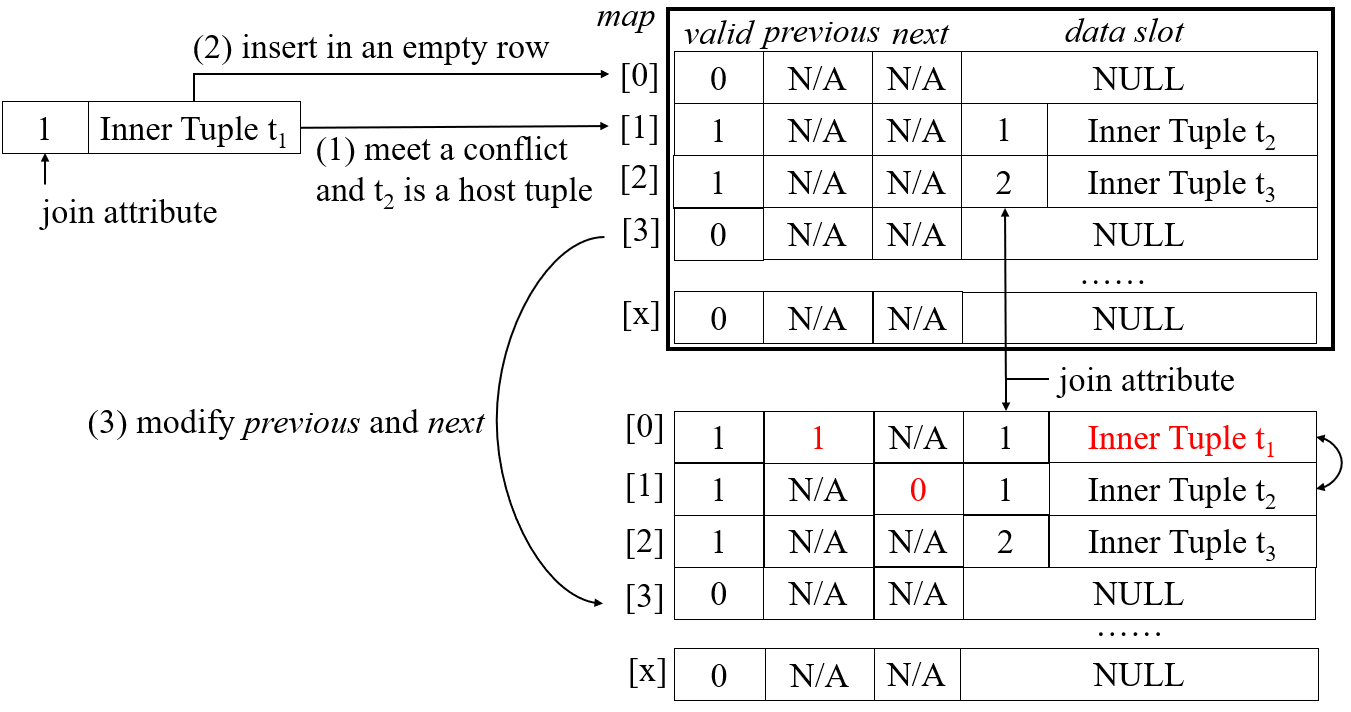
\includegraphics[width=\linewidth]{./pic/Figure18.png}
        \caption{The illustration of condition 2}
        \label{F18}
        \Description{}
    \end{figure}\par
    \textbf{Case 3} (Figure \ref{F19}): If \textit{valid} is 1 and $t_2$ is a ``guest tuple", whose join attribute value does not equal to its row number. We first move $t_2$ to a new empty row, then fit $t_1$ in this row as ``host tuple" and set the \textit{previous} and \textit{next} to $N/A$. Then, we refresh the position of $t_2$ in the list where all members have the same join attribute value with $t_2$.
    \begin{figure}[htb]
        \centering
        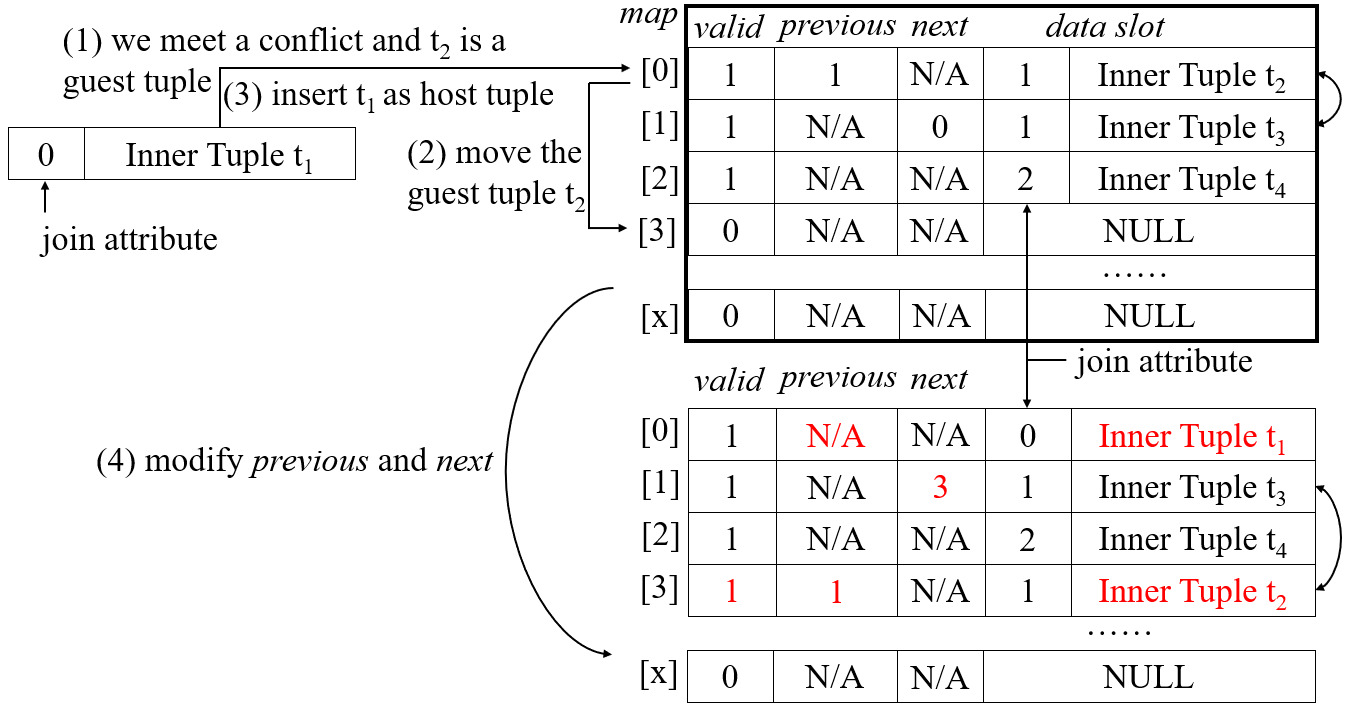
\includegraphics[width=\linewidth]{./pic/Figure19.png}
        \caption{The illustration of condition 3}
        \label{F19}
        \Description{}
    \end{figure}\par
    After introducing how to build \textit{map}, we describe how to return a join result in probe phase. As shown in Figure \ref{F20}, we first fetch an outer tuple, and then we get the join attribute value of outer tuple as row number to fetch the corresponding row in \textit{map}. After we fetch the corresponding row from \textit{map}, we check its \textit{valid word}. If empty, we fetch the next outer tuple and repeat above steps. Otherwise, we check \textit{next} to determine whether there is a list. If $N/A$, which means there is only one tuple has given join attribute value, we return the join result and fetch next outer tuple. If not $N/A$, we not only return the join result, but also fetch the successors that have the same join attribute value by traversing the list.
    \begin{figure}[htb]
        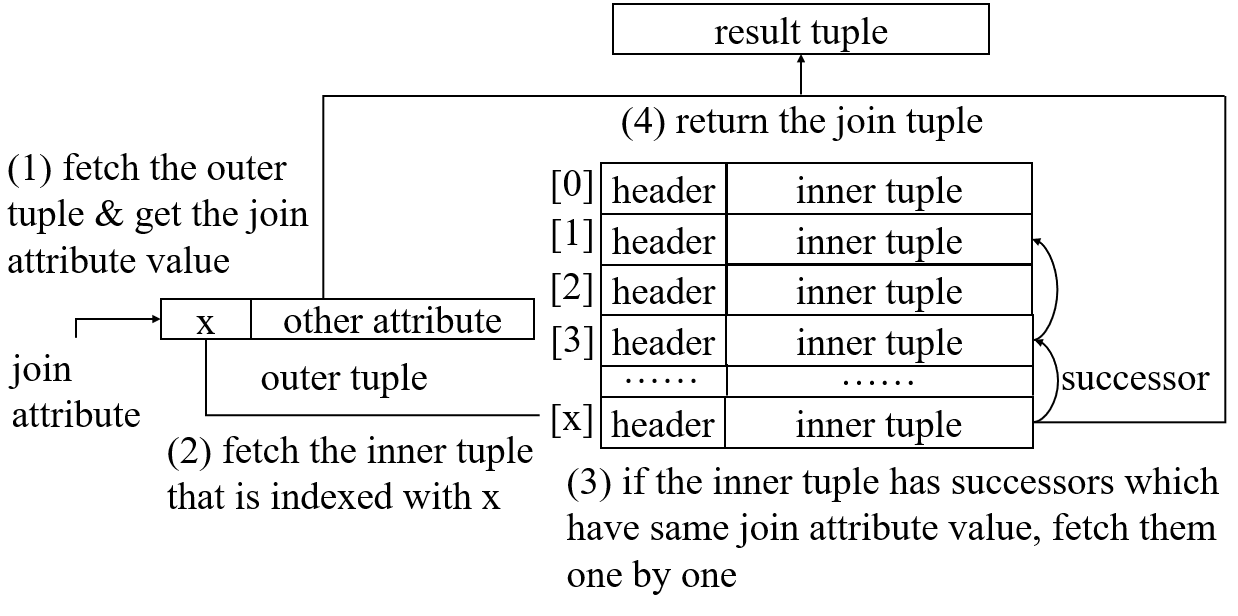
\includegraphics[width=\linewidth]{./pic/Figure20.png}
        \caption{How \textit{directmap join} works}
        \label{F20}
        \Description{}
    \end{figure}\par
    Another problem is how to combine \textit{directmap join} with PostgreSQL optimizer. By our design, whether the optimizer chooses the \textit{directmap join} operator depends on a heuristic judgment and its cost model.\par
    A heuristic judgment is used to control the memory usage, as the size of \textit{map} is no less than the maximum of join attribute, which means \textit{directmap join} sacrifices memory to earn speed. First, we ensure that the inner relation must be a base relation or a subquery result to avoid too much confliction. Then, we check the ratio $t=f_r/n_r$, where $f_r$ is the estimated number of tuples after applying the predicate on inner relation, and $n_r$ is the size of inner relation. As \textit{map} size is no less than the maximum of appeared join attribute values, we use $n_r$ to approximate the \textit{map} size. And $f_r$ equals the number of rows that we actually use in \textit{map}. Hence, the ratio can roughly estimate the ratio of how much memory that we actually use for storage and allocate for \textit{directmap join}, which reflects the memory utilization rate of \textit{directmap join}. If the ratio is less than a threshold, we think it's memory-wasteful to create a \textit{map}, so we abandon the consideration of using \textit{directmap join}.\par
    Second, we set the cost model of \textit{directmap join} by imitating the cost model of \textit{hash join}. As \textit{directmap join} reduced twice memory access to once, we half the fetch cost by CPU. To show our change in fetch cost, we divide the cost of \textit{hash join} by two as the cost of \textit{directmap join}. \label{A3}

\end{document}
\endinput